% 若编译失败,且生成 .synctex(busy) 辅助文件,可能有两个原因:
% 1. 需要插入的图片不存在:Ctrl + F 搜索 'figure' 将这些代码注释/删除掉即可
% 2. 路径/文件名含中文或空格:更改路径/文件名即可

% --------------------- 文章宏包及相关设置 --------------------- %
% >> ------------------ 文章宏包及相关设置 ------------------ << %
% 设定文章类型与编码格式
\documentclass[UTF8]{article}		

% 物理实验报告所需的其它宏包
\usepackage{ulem}   % \uline 下划线支持
\usepackage{circuitikz} % 电路图 tikz 支持
\usepackage{pdfpages}   % 用于导入 pdf 文件
\usepackage{multirow}   % 用于表格合并单元格

% 本 .tex 专属的宏定义
    \def\V{\ \mathrm{V}}
    \def\uV{\ \mu\mathrm{V}}
    \def\mV{\ \mathrm{mV}}
    \def\K{\ \mathrm{K}}
    \def\kV{\ \mathrm{KV}}
    \def\KV{\ \mathrm{KV}}
    \def\MV{\ \mathrm{MV}}
    \def\uA{\ \mu\mathrm{A}}
    \def\mA{\ \mathrm{mA}}
    \def\A{\ \mathrm{A}}
    \def\kA{\ \mathrm{KA}}
    \def\KA{\ \mathrm{KA}}
    \def\MA{\ \mathrm{MA}}
    \def\O{\ \Omega}
    \def\mO{\ \Omega}
    \def\kO{\ \mathrm{K}\Omega}
    \def\KO{\ \mathrm{K}\Omega}
    \def\MO{\ \mathrm{M}\Omega}
    \def\Hz{\ \mathrm{Hz}}
    \def\uF{\ \mu\mathrm{F}}
    \def\mF{\ \mathrm{mF}}
    \def\F{\ \mathrm{F}}
    \def\Re{\mathrm{\,Re}\,}
    \def\Im{\mathrm{\,Im}\,}
    \def\sinc{\mathrm{\,sinc}\,}

% 自定义宏定义
    \def\N{\mathbb{N}}
    \def\F{\mathbb{F}}
    \def\Z{\mathbb{Z}}
    \def\Q{\mathbb{Q}}
    \def\R{\mathbb{R}}
    \def\C{\mathbb{C}}
    \def\T{\mathbb{T}}
    \def\S{\mathbb{S}}
    %\def\A{\mathbb{A}}
    \def\I{\mathscr{I}}
    \def\d{\mathrm{d}}
    \def\p{\partial}


% 导入基本宏包
    \usepackage[UTF8]{ctex}     % 设置文档为中文语言
    \usepackage{hyperref}  % 宏包:自动生成超链接 (此宏包与标题中的数学环境冲突)
    \hypersetup{
        colorlinks=true,    % false:边框链接 ; true:彩色链接
        citecolor={blue},    % 文献引用颜色
        linkcolor={blue},   % 目录 (我们在目录处单独设置),公式,图表,脚注等内部链接颜色
        urlcolor={orange},    % 网页 URL 链接颜色,包括 \href 中的 text
        % cyan 浅蓝色 
        % magenta 洋红色
        % yellow 黄色
        % black 黑色
        % white 白色
        % red 红色
        % green 绿色
        % blue 蓝色
        % gray 灰色
        % darkgray 深灰色
        % lightgray 浅灰色
        % brown 棕色
        % lime 石灰色
        % olive 橄榄色
        % orange 橙色
        % pink 粉红色
        % purple 紫色
        % teal 蓝绿色
        % violet 紫罗兰色
    }
    % \usepackage{docmute}    % 宏包:子文件导入时自动去除导言区,用于主/子文件的写作方式,\include{./51单片机笔记}即可。注:启用此宏包会导致.tex文件capacity受限。
    \usepackage{amsmath}    % 宏包:数学公式
    \usepackage{mathrsfs}   % 宏包:提供更多数学符号
    \usepackage{amssymb}    % 宏包:提供更多数学符号
    \usepackage{pifont}     % 宏包:提供了特殊符号和字体
    \usepackage{extarrows}  % 宏包:更多箭头符号 
    \usepackage{multicol}   % 宏包:支持多栏 

% 文章页面margin设置
    \usepackage[a4paper]{geometry}
        \geometry{top=0.75in}
        \geometry{bottom=0.75in}
        \geometry{left=0.75in}
        \geometry{right=0.75in}   % 设置上下左右页边距
        \geometry{marginparwidth=1.75cm}    % 设置边注距离(注释、标记等)

% 配置数学环境
    \usepackage{amsthm} % 宏包:数学环境配置
    % theorem-line 环境自定义
        \newtheoremstyle{MyLineTheoremStyle}% <name>
            {11pt}% <space above>
            {11pt}% <space below>
            {}% <body font> 默认使用正文字体,  为楷体
            {}% <indent amount>
            {\bfseries}% <theorem head font> 设置标题项为加粗
            {:\ \ }% <punctuation after theorem head>
            {.5em}% <space after theorem head>
            {\textbf{#1}\thmnumber{#2}\ \ (\,\textbf{#3}\,)}% 设置标题内容顺序
        \theoremstyle{MyLineTheoremStyle} % 应用自定义的定理样式
        \newtheorem{LineTheorem}{Theorem.\,}
    % theorem-block 环境自定义
        \newtheoremstyle{MyBlockTheoremStyle}% <name>
            {11pt}% <space above>
            {11pt}% <space below>
            {}% <body font> 使用默认正文字体
            {}% <indent amount>
            {\bfseries}% <theorem head font> 设置标题项为加粗
            {:\\ \indent}% <punctuation after theorem head>
            {.5em}% <space after theorem head>
            {\textbf{#1}\thmnumber{#2}\ \ (\,\textbf{#3}\,)}% 设置标题内容顺序
        \theoremstyle{MyBlockTheoremStyle} % 应用自定义的定理样式
        \newtheorem{BlockTheorem}[LineTheorem]{Theorem.\,} % 使用 LineTheorem 的计数器
    % definition 环境自定义
        \newtheoremstyle{MySubsubsectionStyle}% <name>
            {11pt}% <space above>
            {11pt}% <space below>
            {}% <body font> 使用默认正文字体
            {}% <indent amount>
            {\bfseries}% <theorem head font> 设置标题项为加粗
            {:\\ \indent}% <punctuation after theorem head>
            {0pt}% <space after theorem head>
            {\textbf{#3}}% 设置标题内容顺序
        \theoremstyle{MySubsubsectionStyle} % 应用自定义的定理样式
        \newtheorem{definition}{}

%宏包:有色文本框(proof环境)及其设置
    \usepackage{xcolor}    %设置插入的文本框颜色
    \usepackage[strict]{changepage}     % 提供一个 adjustwidth 环境
    \usepackage{framed}     % 实现方框效果
        \definecolor{graybox_color}{rgb}{0.95,0.95,0.96} % 文本框颜色。修改此行中的 rgb 数值即可改变方框纹颜色,具体颜色的rgb数值可以在网站https://colordrop.io/ 中获得。(截止目前的尝试还没有成功过,感觉单位不一样)(找到喜欢的颜色,点击下方的小眼睛,找到rgb值,复制修改即可)
        \newenvironment{graybox}{%
        \def\FrameCommand{%
        \hspace{1pt}%
        {\color{gray}\vrule width 2pt}%
        {\color{graybox_color}\vrule width 4pt}%
        \colorbox{graybox_color}%
        }%
        \MakeFramed{\advance\hsize-\width\FrameRestore}%
        \noindent\hspace{-4.55pt}% disable indenting first paragraph
        \begin{adjustwidth}{}{7pt}%
        \vspace{2pt}\vspace{2pt}%
        }
        {%
        \vspace{2pt}\end{adjustwidth}\endMakeFramed%
        }

% 外源代码插入设置
    % matlab 代码插入设置
    \usepackage{matlab-prettifier}
        \lstset{style=Matlab-editor}    % 继承 matlab 代码高亮 , 此行不能删去
    \usepackage[most]{tcolorbox} % 引入tcolorbox包 
    \usepackage{listings} % 引入listings包
        \tcbuselibrary{listings, skins, breakable}
        \newfontfamily\codefont{Consolas} % 定义需要的 codefont 字体
        \lstdefinestyle{MatlabStyle_inc}{   % 插入代码的样式
            language=Matlab,
            basicstyle=\footnotesize\ttfamily\codefont,    % ttfamily 确保等宽 
            breakatwhitespace=false,
            breaklines=true,
            captionpos=b,
            keepspaces=true,
            numbers=left,
            numbersep=15pt,
            showspaces=false,
            showstringspaces=false,
            showtabs=false,
            tabsize=2,
            xleftmargin=15pt,   % 左边距
            %frame=single, % single 为包围式单线框
            frame=shadowbox,    % shadowbox 为带阴影包围式单线框效果
            %escapeinside=``,   % 允许在代码块中使用 LaTeX 命令 (此行无用)
            %frameround=tttt,    % tttt 表示四个角都是圆角
            framextopmargin=0pt,    % 边框上边距
            framexbottommargin=0pt, % 边框下边距
            framexleftmargin=5pt,   % 边框左边距
            framexrightmargin=5pt,  % 边框右边距
            rulesepcolor=\color{red!20!green!20!blue!20}, % 阴影框颜色设置
            %backgroundcolor=\color{blue!10}, % 背景颜色
        }
        \lstdefinestyle{MatlabStyle_src}{   % 插入代码的样式
            language=Matlab,
            basicstyle=\small\ttfamily\codefont,    % ttfamily 确保等宽 
            breakatwhitespace=false,
            breaklines=true,
            captionpos=b,
            keepspaces=true,
            numbers=left,
            numbersep=15pt,
            showspaces=false,
            showstringspaces=false,
            showtabs=false,
            tabsize=2,
        }
        \newtcblisting{matlablisting}{
            %arc=2pt,        % 圆角半径
            % 调整代码在 listing 中的位置以和引入文件时的格式相同
            top=0pt,
            bottom=0pt,
            left=-5pt,
            right=-5pt,
            listing only,   % 此句不能删去
            listing style=MatlabStyle_src,
            breakable,
            colback=white,   % 选一个合适的颜色
            colframe=black!0,   % 感叹号后跟不透明度 (为 0 时完全透明)
        }
        \lstset{
            style=MatlabStyle_inc,
        }

% table 支持
    \usepackage{booktabs}   % 宏包:三线表
    \usepackage{tabularray} % 宏包:表格排版
    \usepackage{longtable}  % 宏包:长表格

% figure 设置
    \usepackage{graphicx}  % 支持 jpg, png, eps, pdf 图片 
    \usepackage{svg}       % 支持 svg 图片
        \svgsetup{
            % 指向 inkscape.exe 的路径
            inkscapeexe = C:/aa_MySame/inkscape/bin/inkscape.exe, 
            % 一定程度上修复导入后图片文字溢出几何图形的问题
            inkscapelatex = false                 
        }
    \usepackage{subcaption} % 用于子图和小图注  

% 图表进阶设置
    \usepackage{caption}    % 图注、表注
        \captionsetup[figure]{name=图}  
        \captionsetup[table]{name=表}
        \captionsetup{
            labelfont=bf, % 设置标签为粗体
            textfont=bf,  % 设置文本为粗体
            font=small  
        }
    \usepackage{float}     % 图表位置浮动设置 
    \usepackage{etoolbox} % 用于保证图注表注的数学字符为粗体
        \AtBeginEnvironment{figure}{\boldmath} % 图注中的数学字符为粗体
        \AtBeginEnvironment{table}{\boldmath}  % 表注中的数学字符为粗体
        \AtBeginEnvironment{tabular}{\unboldmath}   % 保证表格中的数学字符不受额外影响

% 圆圈序号自定义
    \newcommand*\circled[1]{\tikz[baseline=(char.base)]{\node[shape=circle,draw,inner sep=0.8pt, line width = 0.03em] (char) {\bfseries #1};}}   % TikZ solution

% 列表设置
    \usepackage{enumitem}   % 宏包:列表环境设置
        \setlist[enumerate]{
            label=(\arabic*) ,   % 设置序号样式为加粗的 (1) (2) (3)
            ref=\arabic*, % 如果需要引用列表项,这将决定引用格式(这里仍然使用数字)
            itemsep=0pt, parsep=0pt, topsep=0pt, partopsep=0pt, leftmargin=3.5em} 
        \setlist[itemize]{itemsep=0pt, parsep=0pt, topsep=0pt, partopsep=0pt, leftmargin=3.5em}
        \newlist{circledenum}{enumerate}{1} % 创建一个新的枚举环境  
        \setlist[circledenum,1]{  
            label=\protect\circled{\arabic*}, % 使用 \arabic* 来获取当前枚举计数器的值,并用 \circled 包装它  
            ref=\arabic*, % 如果需要引用列表项,这将决定引用格式(这里仍然使用数字)
            itemsep=0pt, parsep=0pt, topsep=0pt, partopsep=0pt, leftmargin=3.5em
        }  

% 其它设置
    % 脚注设置
        \renewcommand\thefootnote{\ding{\numexpr171+\value{footnote}}}
    % 参考文献引用设置
        \bibliographystyle{unsrt}   % 设置参考文献引用格式为unsrt
        \newcommand{\upcite}[1]{\textsuperscript{\cite{#1}}}     % 自定义上角标式引用
    % 文章序言设置
        \newcommand{\cnabstractname}{序言}
        \newenvironment{cnabstract}{%
            \par\Large
            \noindent\mbox{}\hfill{\bfseries \cnabstractname}\hfill\mbox{}\par
            \vskip 2.5ex
            }{\par\vskip 2.5ex}

% 文章默认字体设置
    \usepackage{fontspec}   % 宏包:字体设置
        \setmainfont{SimSun}    % 设置中文字体为宋体字体
        \setCJKmainfont[AutoFakeBold=3]{SimSun} % 设置加粗字体为 SimSun 族,AutoFakeBold 可以调整字体粗细
        \setmainfont{Times New Roman} % 设置英文字体为Times New Roman

% 各级标题自定义设置
    \usepackage{titlesec}   
        % section标题自定义设置 
        \titleformat{\section}[hang]{\normalfont\Large\bfseries\boldmath}{\thesection}{8pt}{}
        % subsection 标题自定义设置
        \titleformat{\subsection}[hang]{\normalfont\large\bfseries\boldmath}{\thesubsection}{8pt}{}
        \titlespacing*{\subsection}{0pt}{10pt}{6pt} % 控制上下间距


% --------------------- 文章宏包及相关设置 --------------------- %
% >> ------------------ 文章宏包及相关设置 ------------------ << %


% ------------------------ 文章信息区 ------------------------ %
% ------------------------ 文章信息区 ------------------------ %

% 每次实验报告需要修改的信息有:
% 1. 实验名称 
% 2. 实验日期 
% 3. 实验地点 
% 4. 左上角页眉 
% 5. 指导教师 

% 页眉页脚设置
\usepackage{fancyhdr}   %宏包:页眉页脚设置
    \pagestyle{fancy}
    \fancyhf{}
    \cfoot{\thepage}
    \renewcommand\headrulewidth{1pt}
    \renewcommand\footrulewidth{0pt}
    \rhead{\bfseries \large {\color{red} 分组序号: 2-05}}
    \chead{《基础物理实验》实验报告,\ 丁毅,\ 2023K8009908031}
    \lhead{\small Ex.03 驻波实验 (2024.12.03)}
\begin{document}


\begin{center}\large
    \vspace*{-0.9cm}
    \noindent{\huge\bfseries《\ \ 基\ \ 础\ \ 物\ \ 理\ \ 实\ \ 验\ \ \ 》\ \ 实\ \ 验\ \ 报\ \ 告 }
    \\\vspace{0.5mm}
    \noindent{
    {\bfseries 
    实验名称:\uline{\hspace{0.3cm} 弦上驻波及介质中的声速测量 \hspace{0.3cm}}
    }\hspace{0.4cm}
    指导教师:\uline{\hspace{0.4cm} \ 王智茂 wangzm@ihep.ac.cn\ \hspace{0.4cm}}
    }
    \\\vspace{0.1cm}
    \noindent
    {
    姓名:\uline{\,\,\,丁毅\,\,\,}\hspace{0.2cm}
    学号:\uline{\,\,\,{ 2023K8009908031}\,\,\,}\hspace{0.2cm}
    班级/专业:\uline{\,\,\,{2308/电子信息}\,\,\,}\hspace{0.2cm}
    分组序号:\uline{\,\,\,{2-05}\,\,\,}
    }
    \\\vspace{0.1cm}
    \noindent{
    实验日期:\uline{\,\,{ 2024.12.03}\,\,}\hspace{0.2cm}
    实验地点:\uline{\,\,\,教学楼{ 721}\,\,\,}\hspace{0.2cm}
    是否调课/补课:\uline{\hspace{0.26cm}否 \hspace{0.26cm}}\hspace{0.2cm}
    成绩:\uline{\hspace{2cm}}
    }
\end{center}
\vspace{-0.5cm}
\noindent\rule{\textwidth}{0.075em}   % 分割线
\vspace{-1.1cm}

% 目录
%\zihao{-5}
\setcounter{tocdepth}{3}  % 目录深度为 2(不显示 subsubsection)
\noindent\tableofcontents\thispagestyle{fancy}   % 显示页码、页眉等
\newpage
\rhead{\bfseries\small 分组序号: 2-05}
\zihao{5}
% ------------------------ 文章信息区 ------------------------ %
% ------------------------ 文章信息区 ------------------------ %


%% 下面是正文内容

\section{第一部分:弦上驻波实验}

\subsection{实验目的}
\begin{enumerate}
\item 观察在两端固定的弦线上形成的驻波现象,了解弦线达到共振和形成稳定驻波的条件;
\item 测定弦线上横波的传播速度;
\item 用实验的方式确定弦线作受迫振动时共振频率和半波长个数$ n $、弦线有效长度、张力及线密度之间的关系;
\item 用对数作图和最小二乘法对共振频率与张力关系的实验结果作线性拟合,处理数据,并给出结论。
\end{enumerate}



\subsection{实验器材}
本实验主要实验装置有弦音计、信号发生器、双踪示波器三部分。此外还有天平等测量工具。
\begin{enumerate}
\item 弦音计由吉他弦、固定吉他弦的支架和基座、琴码、砝码支架、驱动线圈、探测线圈和砝码等组成。驱动线圈和探测线圈是本装置的重要部分,其中驱动线圈通过信号发生器提供一定频率的功率信号产生交变磁力,使得金属弦线振动;探测线圈将弦线的振动转换为电信号,通过示波器进行观察。
\item 信号发生器为低频功率信号发生器,其输出信号的频率从$ 10\,\mathrm{Hz} $到$ 1\,\mathrm{kHz} $,用于为驱动线圈提供上述频率范围中具有一定功率的正弦信号。
\item 双踪示波器用于观察信号源的波形并显示由探测线圈接收到的弦线振动的波形,进而可以及时观察弦线的振动现象。
\end{enumerate}

\begin{figure}[H]
    \centering
    \begin{tikzpicture}
        \filldraw[black,fill opacity=0.5] (0,1)--(0.7,1)--(0.9,0.8)--(1.1,0.8)--(1.3,1)--(1.7,1)--(1.9,0.8)--(2.1,0.8)--(2.3,1)--(2.7,1)--(2.9,0.8)--(3.1,0.8)--(3.3,1)--(3.7,1)--(3.9,0.8)--(4.1,0.8)--(4.3,1)--(4.7,1)--(4.9,0.8)--(5.1,0.8)--(5.3,1)--(6,1)--(6,0.5)--(0,0.5)--(0,1)--cycle;
        \draw[dashed] (1,1.5)--(1,-0.5);
        \draw[dashed] (2,2)--(2,-0.5);
        \draw[dashed] (3,2.5)--(3,-0.5);
        \draw[dashed] (4,3)--(4,-0.5);
        \draw[dashed] (5,3.5)--(5,-0.5);
        \draw[dashed] (0.7,-1) rectangle (1.3,-0.5);
        \draw[dashed] (1.7,-1) rectangle (2.3,-0.5);
        \draw[dashed] (2.7,-1) rectangle (3.3,-0.5);
        \draw[dashed] (3.7,-1) rectangle (4.3,-0.5);
        \draw[dashed] (4.7,-1) rectangle (5.3,-0.5);
        \node[below left] at(1,0.5) {1};
        \node[below left] at(2,0.5) {2};
        \node[below left] at(3,0.5) {3};
        \node[below left] at(4,0.5) {4};
        \node[below left] at(5,0.5) {5};
        \draw[->] (1,1.5)--(1.6,1.5) node[right]{$ 1mg $};
        \draw[->] (2,2)--(3.2,2) node[right]{$ 2mg $};
        \draw[->] (3,2.5)--(4.8,2.5) node[right]{$ 3mg $};
        \draw[->] (4,3)--(6.4,3) node[right]{$ 4mg $};
        \draw[->] (5,3.5)--(8,3.5) node[right]{$ 5mg $};
        \draw (-4,-1) rectangle (0,3);
        \node at(-2,1) {弦音计};
    \end{tikzpicture}
    \caption{弦音计砝码在不同槽位对弦线的拉力}
\end{figure}

\subsection{实验原理}
将一弦线两端固定,在一端附近使得弦线作振幅恒定的连续简谐振动,从而将有连续的横波波列从该端向另一端传播,前进波传播到另一端时即会发生反射,回到原端点时再次反射,如此不断重复下去。弦线上既有前进波,又有无数的反射波。如果弦线的长度与波长之间满足某种关系,使得前进波与许多反射波都具有相同的相位时,弦线上各点作振幅各自恒定的简谐振动。那么弦线上有些点振动振幅最大,成为波腹;有些点的振幅为零,成为波节,形成驻波现象。

\begin{figure}[!h]
    \centering
    \begin{tikzpicture}
        \draw [domain=0:4*pi,samples=1000,thick] plot (\x,{sin(2*\x r)});
        \draw [domain=0:4*pi,samples=1000,thick,dashed] plot (\x,{-sin(2*\x r)});
        \draw [->] (pi,-2.5)node[below]{波节}--(pi,-0.5);
        \draw [->] (2.75*pi,-2.5)node[below]{波腹}--(2.75*pi,-1.2);
        \draw [ultra thick] (0,-1.2)--(0,1.2);
        \draw [ultra thick] (4*pi,-1.2)--(4*pi,1.2);
    \end{tikzpicture}
    \caption{驻波现象示意图}
\end{figure}

相邻两波节(或波腹)的间隔距离$ D $为波长$ \lambda $的一半,称为半波长,即$ D=\frac\lambda2 $。由于弦线两端固定,故而弦线两端均为波节,那么弦线长度应为半波长的整数倍,记弦线长度为$ L $,则
\begin{equation}
L=nD=\frac{n\lambda}{2},\qquad n=1,2,3,\cdots
\end{equation}

设振动频率为$ f $,则横波沿弦线的传播速度为$ v=f\lambda $。根据波动理论,记拉紧的弦上张力为$ T $,弦线线密度为$ \mu $,波在传播方向的位置坐标为$ x $,振动位移为$ y $,那么沿弦线传播的横波应满足:
\begin{equation}
\frac{\partial^2y}{\partial t^2}=\frac{T\partial^2y}{\mu\partial x^2},\qquad\frac{\partial^2y}{\partial t^2}=v^2\frac{\partial^2y}{\partial x^2}
\end{equation}
进而可以得到波的传播速度满足
\begin{equation}
v=\sqrt{\frac T\mu}
\end{equation}
对比其与$ v=f\lambda $之间的差异,分析理论值与测量值间的区别。

此外频率与张力、线密度间的关系可求得为
\begin{equation}
f=\frac1\lambda\sqrt{\frac T\mu}
\end{equation}
对上式两边取对数,则有
\begin{equation}
\ln f=\frac12\ln T-\frac12\ln\mu-\ln\lambda
\end{equation}

\subsection{实验内容}
\begin{enumerate}
\item 认识和调节仪器;
测定所用弦线的线密度。用天平测定弦线\footnote{选用与所用弦线直径相同、只取吉他弦中段约70-80\,cm的专用样品,而非从弦音计上取下弦线进行测量。}的质量$ m $,并测量弦线长$ L $,则线密度为
\begin{equation}
\mu=\frac mL
\end{equation}

\item 观察弦线上的驻波。固定弦上张力$ T $与波的有效长度$ L $,调节信号发生器的输出频率,观察在两端固定的弦线上形成的有$ n\;(n=1,2,3,\cdots) $个波腹的稳定驻波。
\item 测定弦线上横波的传播速度。先测得张力$ T $与线密度$ \mu $,根据$ v=\sqrt{\frac T\mu} $测得横波传播速度。然后测出共振频率$ f $,波的有效长度$ L $,根据$ \lambda=\frac{2L}{n} $求得波长,再利用$ v=\lambda f $计算得到横波传播速度。比较两种方法得到的实验结果。
\item 固定弦线线密度与弦线张力,确定弦线作受迫振动时的共振频率(只取基频,即$ n=1 $)与弦线有效长度之间的关系,并记录数据。
\item 固定弦线线密度与弦线有效长度,确定弦线作受迫振动时的共振频率(只取基频,即$ n=1 $)与张力之间的关系,并记录数据。
\item 固定弦线张力、弦线有效长度,确定弦线作受迫振动时的共振频率(只取基频,即$ n=1 $)与弦线线密度之间的关系,并记录数据。
\end{enumerate}

\subsection{实验结果与数据处理}
\subsubsection{线密度测定}
虽与线密度测量无关,但后续实验探究频率与线密度关系时,需使用不同粗细琴弦得到的结果,故测量直径以便区分各弦。
\begin{table}[H]\centering
    %\renewcommand{\arraystretch}{1.5} % 调整行间距为 1.5 倍
    %\setlength{\tabcolsep}{1.5mm} % 调整列间距
    \caption{所用弦线的几何与质量参数}
    \label{所用弦线的几何与质量参数}
\begin{tabular}{cccccccccc}\toprule
    弦号 & 质量 (g) & 长度 (mm) & 直径 (mm) & 线密度 $\mathrm{g\cdot m^{-1}}$ \\
    \midrule
    6 & 0.119 & 32.5 &	0.883 &	3.662 \\
    \bottomrule
\end{tabular}
\end{table}


\subsubsection{波速的测量}
将琴码放置于150\,mm和650\,mm处,则弦线有效长度$ L=500\,\mathrm{mm} $,不同频率$ f_n\,(n=1,2,3) $对应的波长$ \lambda=\frac{2L}{n} $,故而$ f_1,f_2,f_3 $ 对应波速公式分别为 $ v_1=2Lf_1,\,v_2=Lf_2,\,v_3=\frac{2Lf_3}{3} $,取平均值即为 $v_{\text{expe}} = \frac{1}{3}\left(v_1 + v_2 + v_3\right)$。我所使用的砝码质量为 $m = 508.02 \ \mathrm{g}$,取 $g = 9.83 \ \mathrm{m\cdot s^{-2}}$,数据与结果汇总如下:
\begin{table}[H]\centering
    %\renewcommand{\arraystretch}{1.5} % 调整行间距为 1.5 倍
    %\setlength{\tabcolsep}{1.5mm} % 调整列间距
    \caption{不同张力下波速的测量}
    \label{不同张力下波速的测量}
\resizebox{\columnwidth}{!}{
    \begin{tabular}{cccccccccc}\toprule
        砝码位置 & 张力 $T$ (N) & $f_1$ (Hz) & $f_2$ (Hz) & $f_3$ (Hz) & 实验 $v_{\text{expe}}$ ($\mathrm{m\cdot s^{-1}}$) & 理论 $v_{\text{theo}}$ ($\mathrm{m\cdot s^{-1}}$) & 相对误差 $\eta$\\
        \midrule
        2 & 4.9938 & 38.33 & 76.84  &116.40 & 36.9760 & 36.9282 & - 0.1293 \%\\
        3 & 7.4908 & 49.25 & 98.73  &148.24 & 47.3691 & 45.2276 & - 4.5208 \%\\
        4 & 9.9877 & 56.56 & 113.21 &169.87 & 54.3323 & 52.2243 & - 3.8797 \%\\
        \bottomrule
    \end{tabular}
}
\end{table}
\begin{figure}[H]\centering
\begin{subfigure}[b]{0.5\columnwidth}\centering
    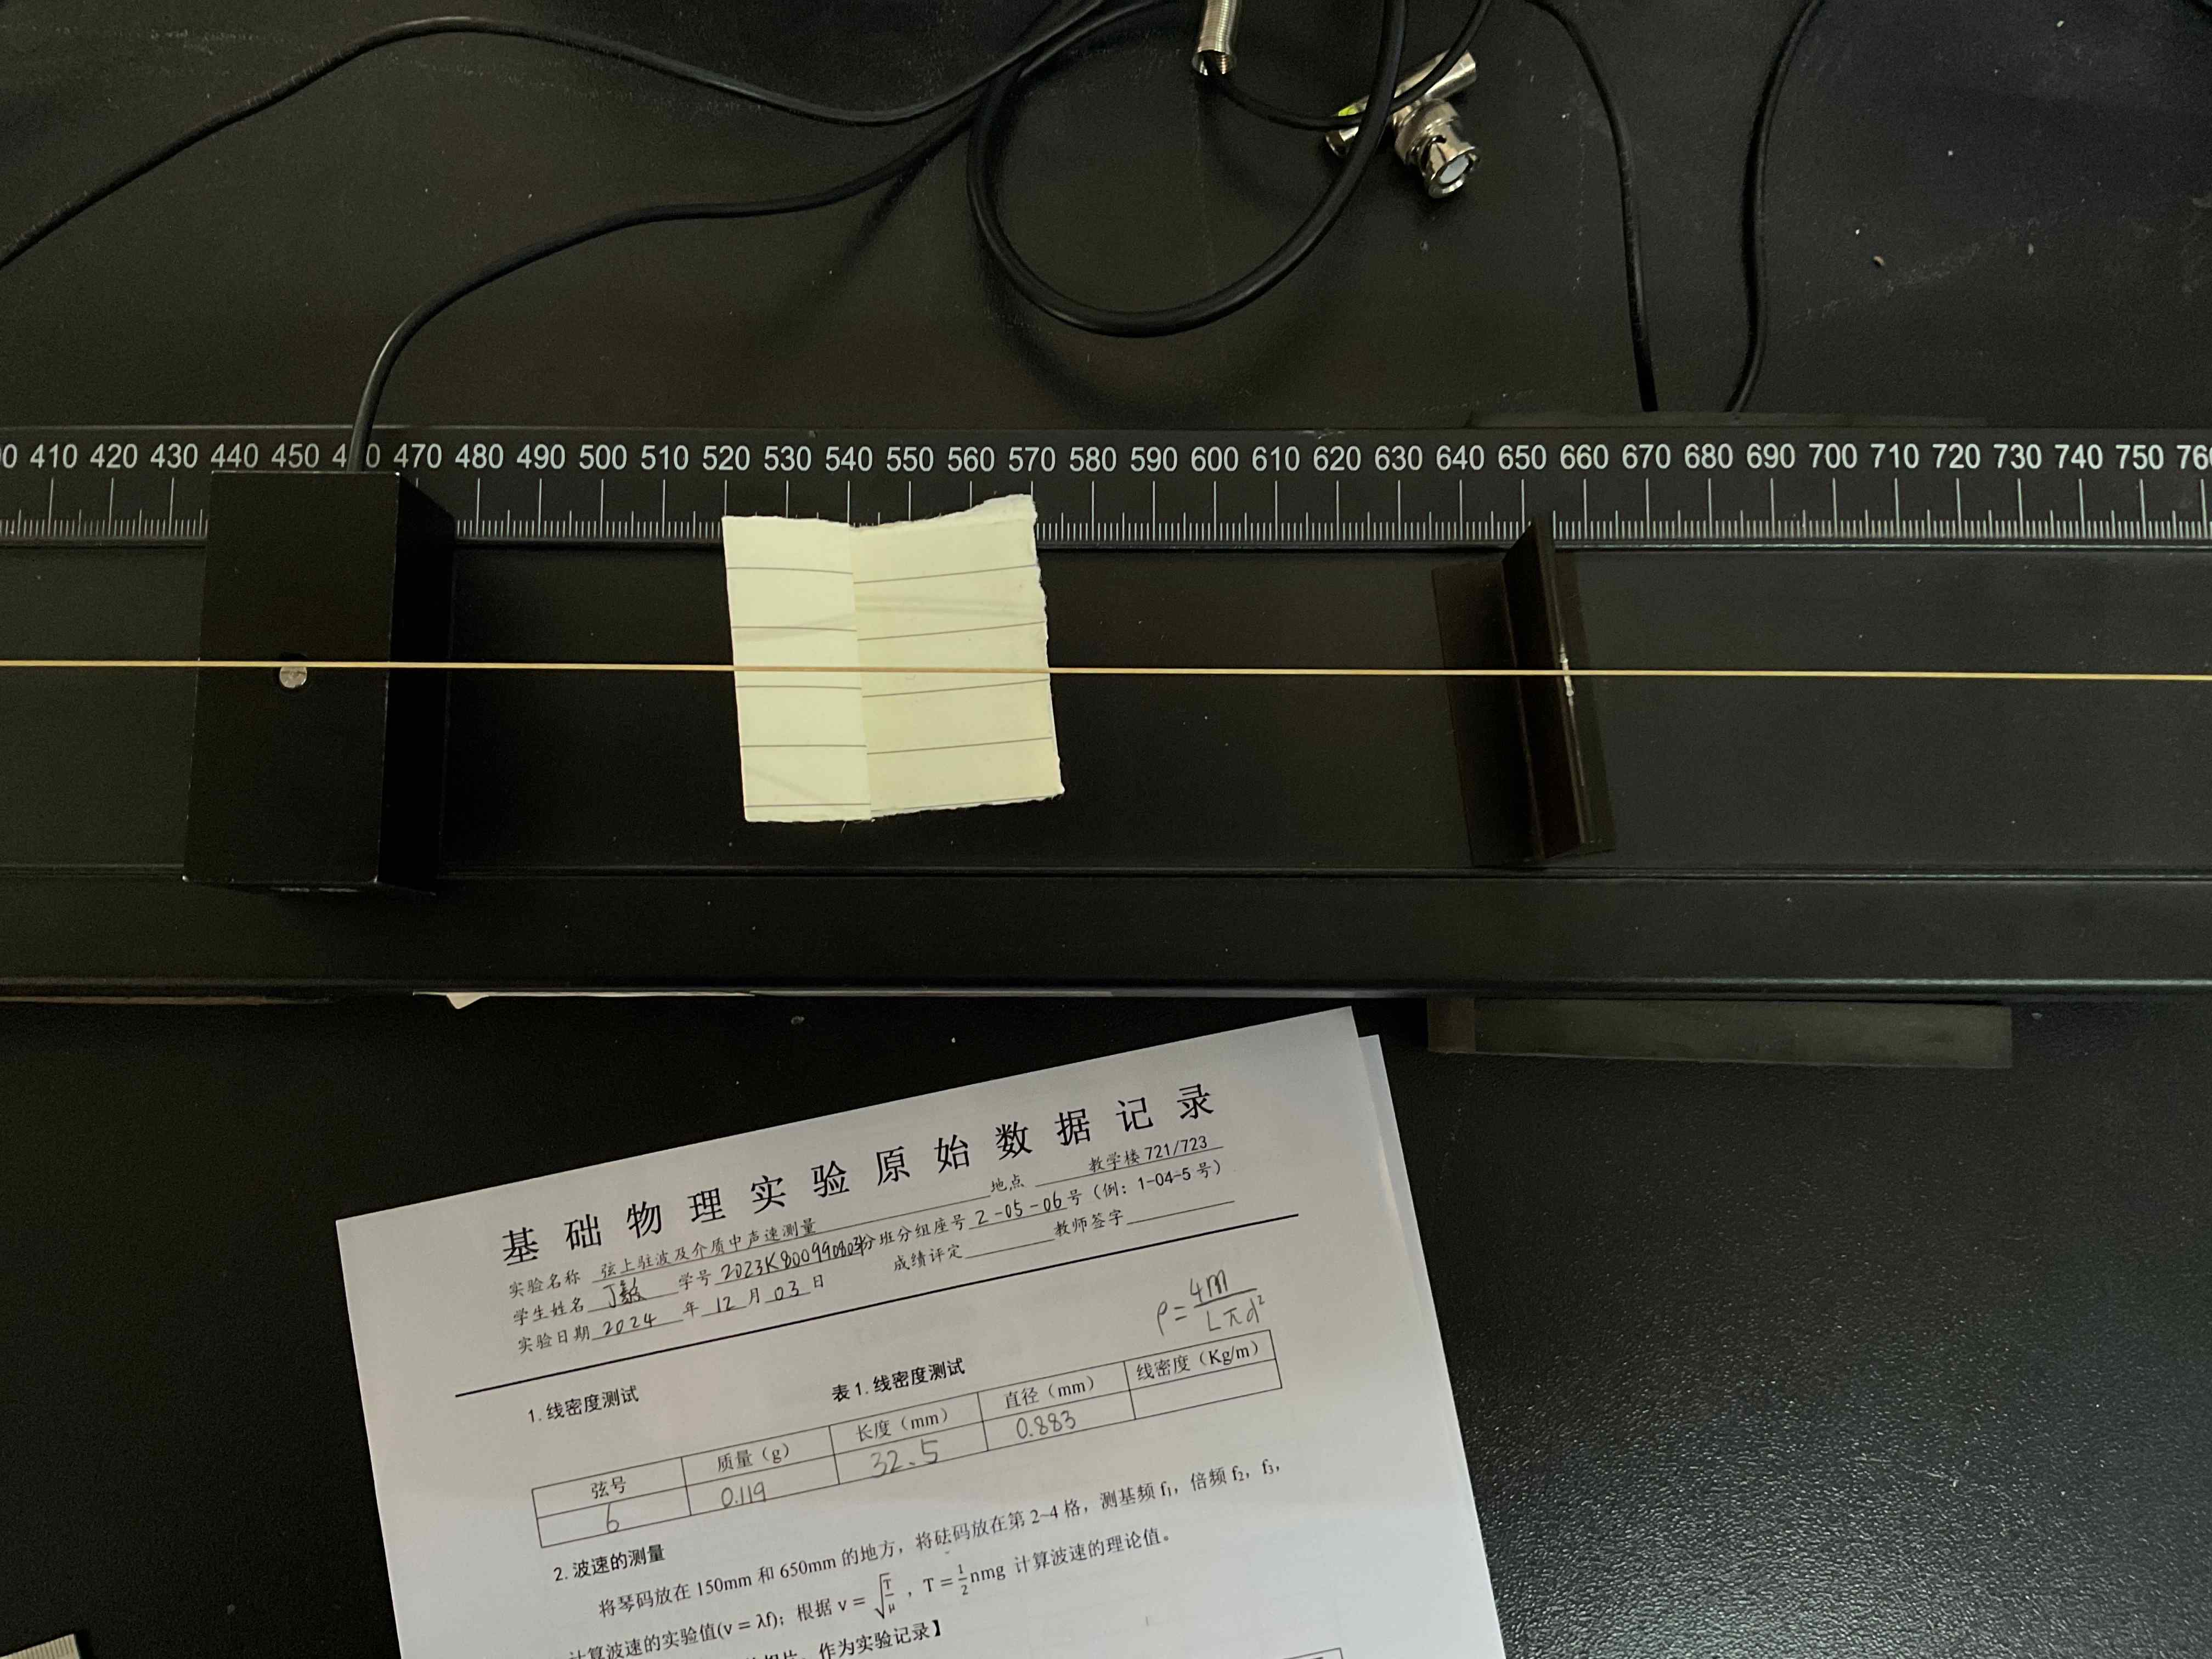
\includegraphics[height=170pt]{assets/波速测量 波节.jpg}
    \caption{波节记录}
\end{subfigure}\hfill
\begin{subfigure}[b]{0.5\columnwidth}\centering
    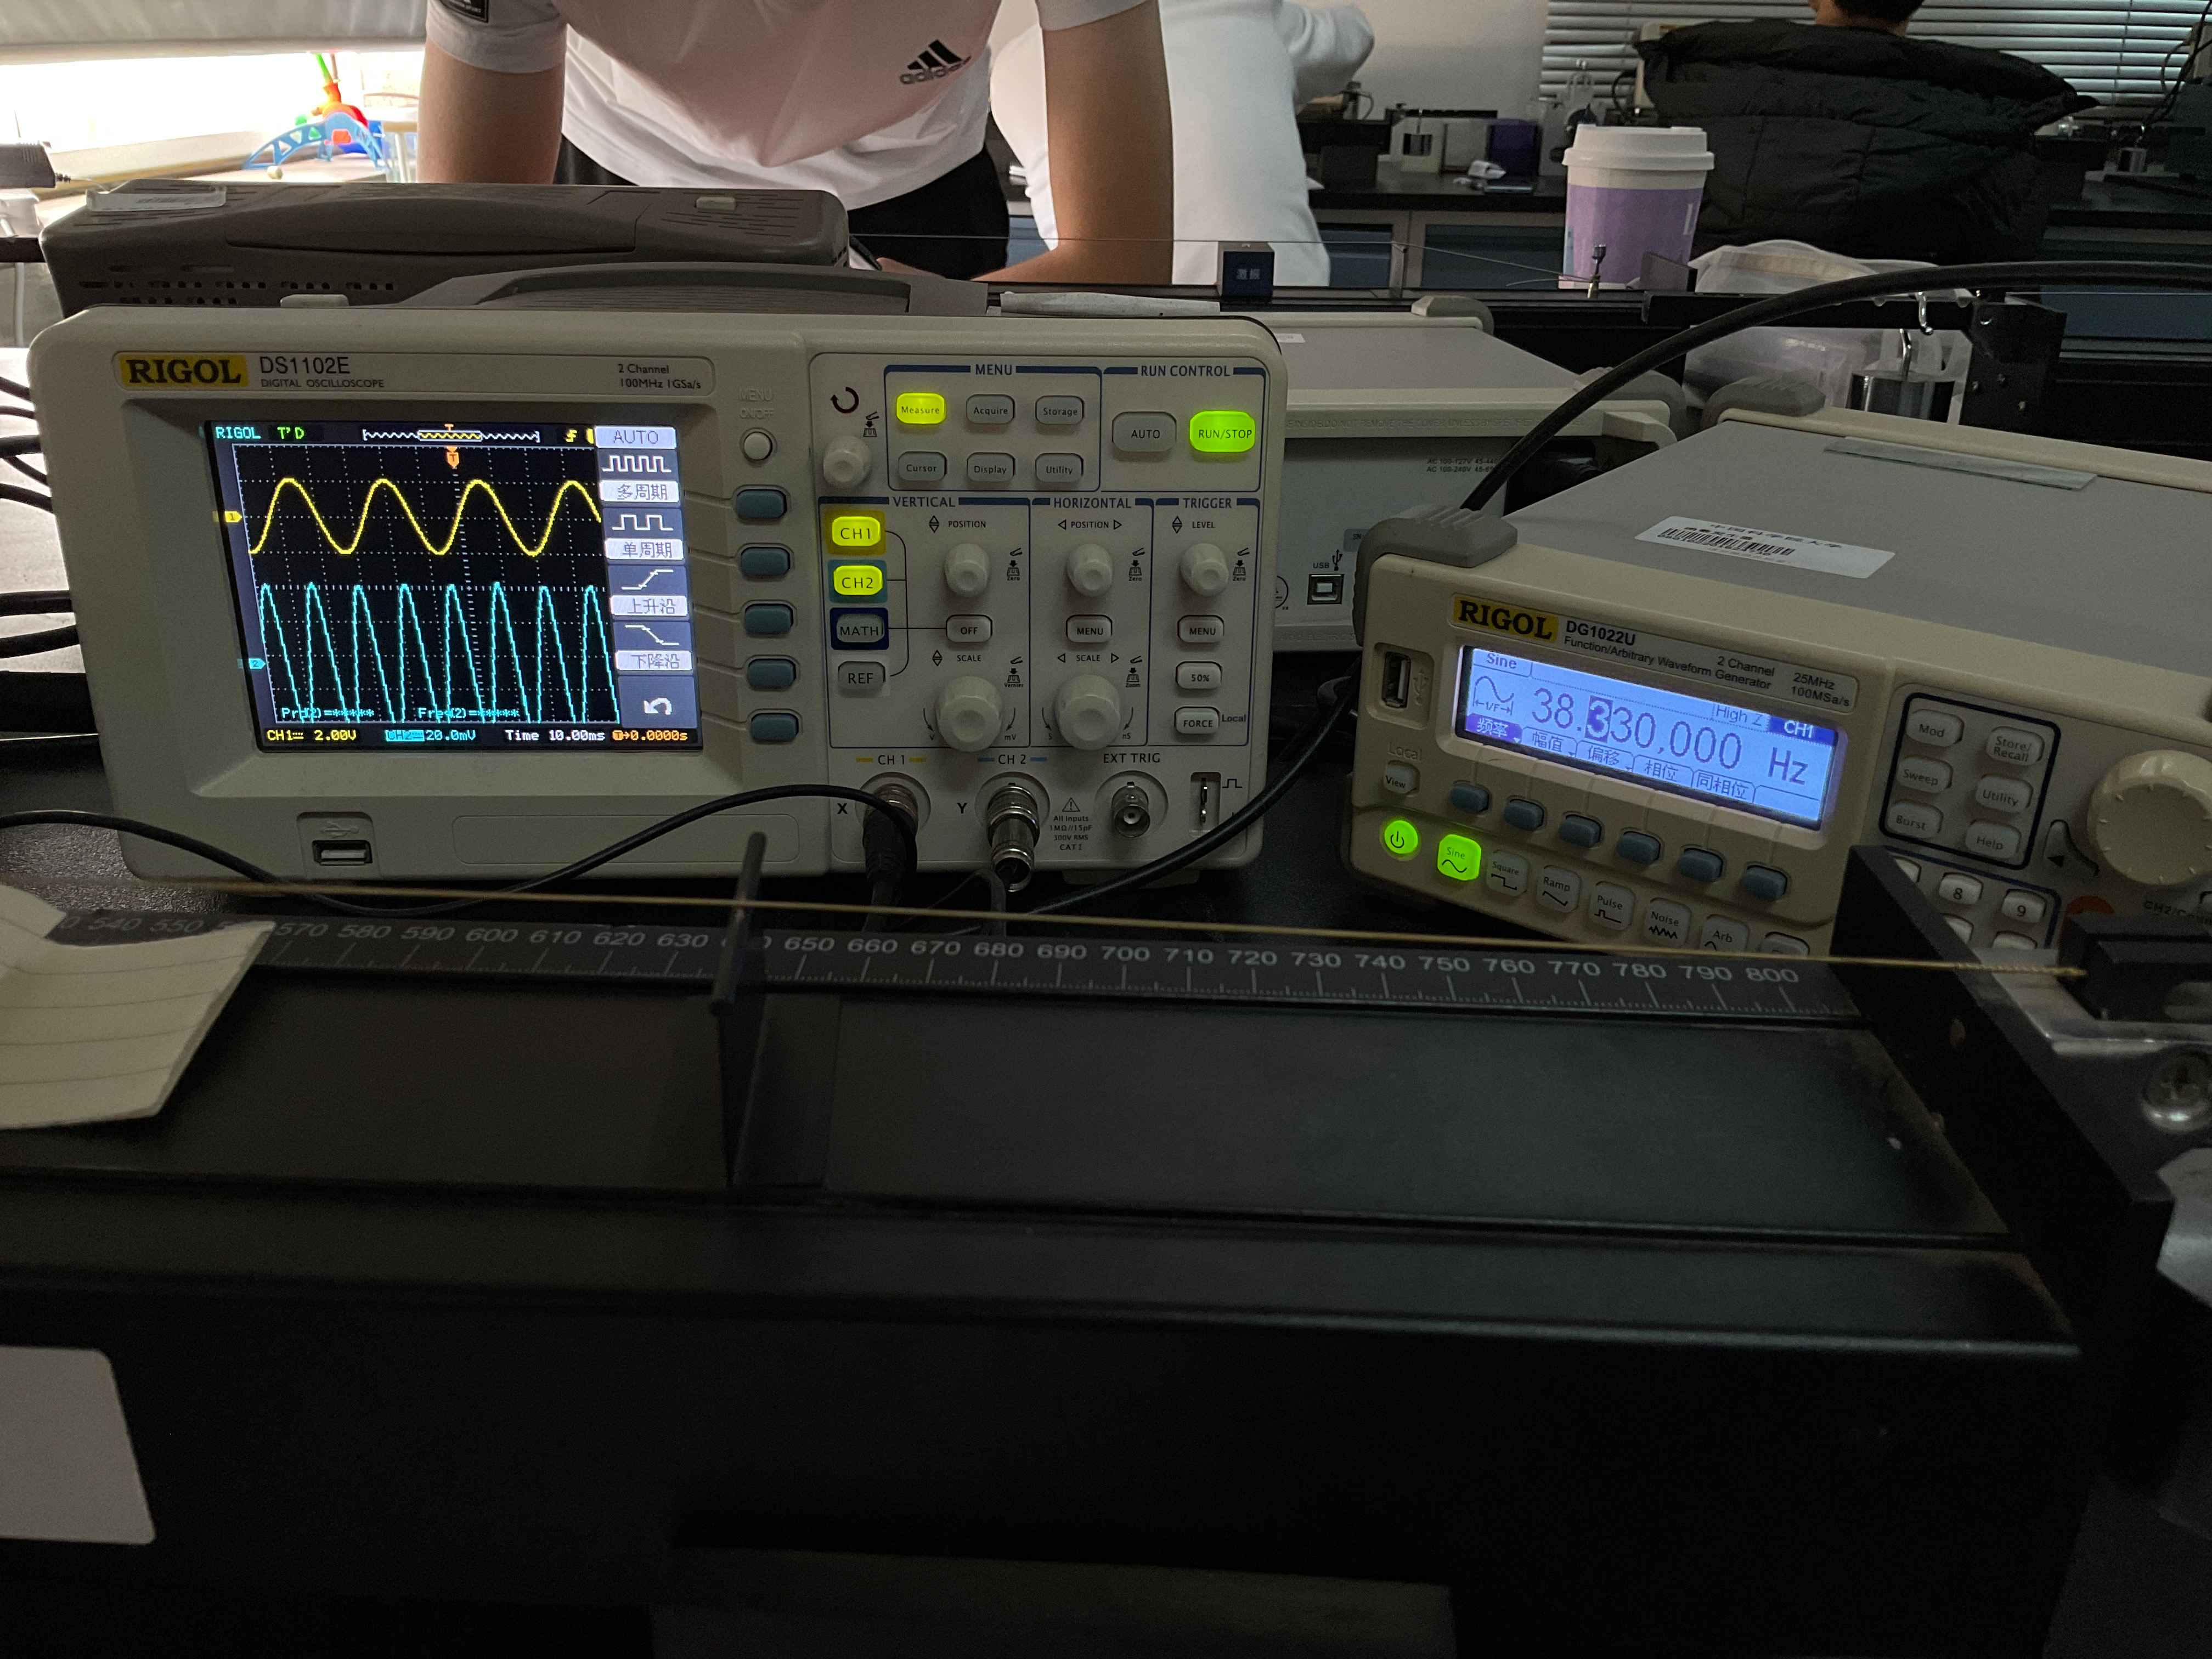
\includegraphics[height=170pt]{assets/波速测量 示波器.jpg}
    \caption{示波器记录}
\end{subfigure}
\caption{波速测量实验照片}
\end{figure}
可见在误差允许范围内两种方法得到的波速大小可看作相等。


\subsubsection{频率与有效长度的关系}
将砝码放在第2格,改变有效长度 $L$(即波长 $\lambda$),测量基频$ f_1 $,数据实验数据如表 \ref{不同有效长度下的基频} 所示。
\begin{table}[H]\centering
    %\renewcommand{\arraystretch}{1.5} % 调整行间距为 1.5 倍
    %\setlength{\tabcolsep}{1.5mm} % 调整列间距
    \caption{不同有效长度下的基频}
    \label{不同有效长度下的基频}
\begin{tabular}{cccccccccc}\toprule
    有效长度 $L$ (m) & 640.00 & 480.00 & 320.00 & 240.00 & 160.00 \\
    \midrule
    基频 $f_1$ & 29.16  & 39.28  & 58.90  & 85.71  & 130.46 \\
    $\ln L$ & 6.4615  &  6.1738  &  5.7683  &  5.4806  &  5.0752 \\
    $\ln f_1$ & 3.3728  &  3.6707  &  4.0758  &  4.4510  &  4.8711 \\
    \bottomrule
\end{tabular}
\end{table}
根据实验数据,在 Matlab 中用最小二乘法求出拟合直线,如图 \ref{有效长度与基频的线性拟合} 所示,其中拟合直线为:
\begin{equation}
y = -1.089 \,x + 10.39,\quad x = \ln L,\ y = \ln f
\end{equation}
由图和拟合直线斜率$ k=-1.089\approx-1 $可知,在误差允许范围内可以认为$ \ln f_1=-\ln L+C $($ C $为常数),即$ f_1\propto\frac1L $,又由于$ L\propto\lambda $,故而实际验证的物理规律为$ f_1\propto\lambda_1 $。



\begin{figure}[H]\centering
    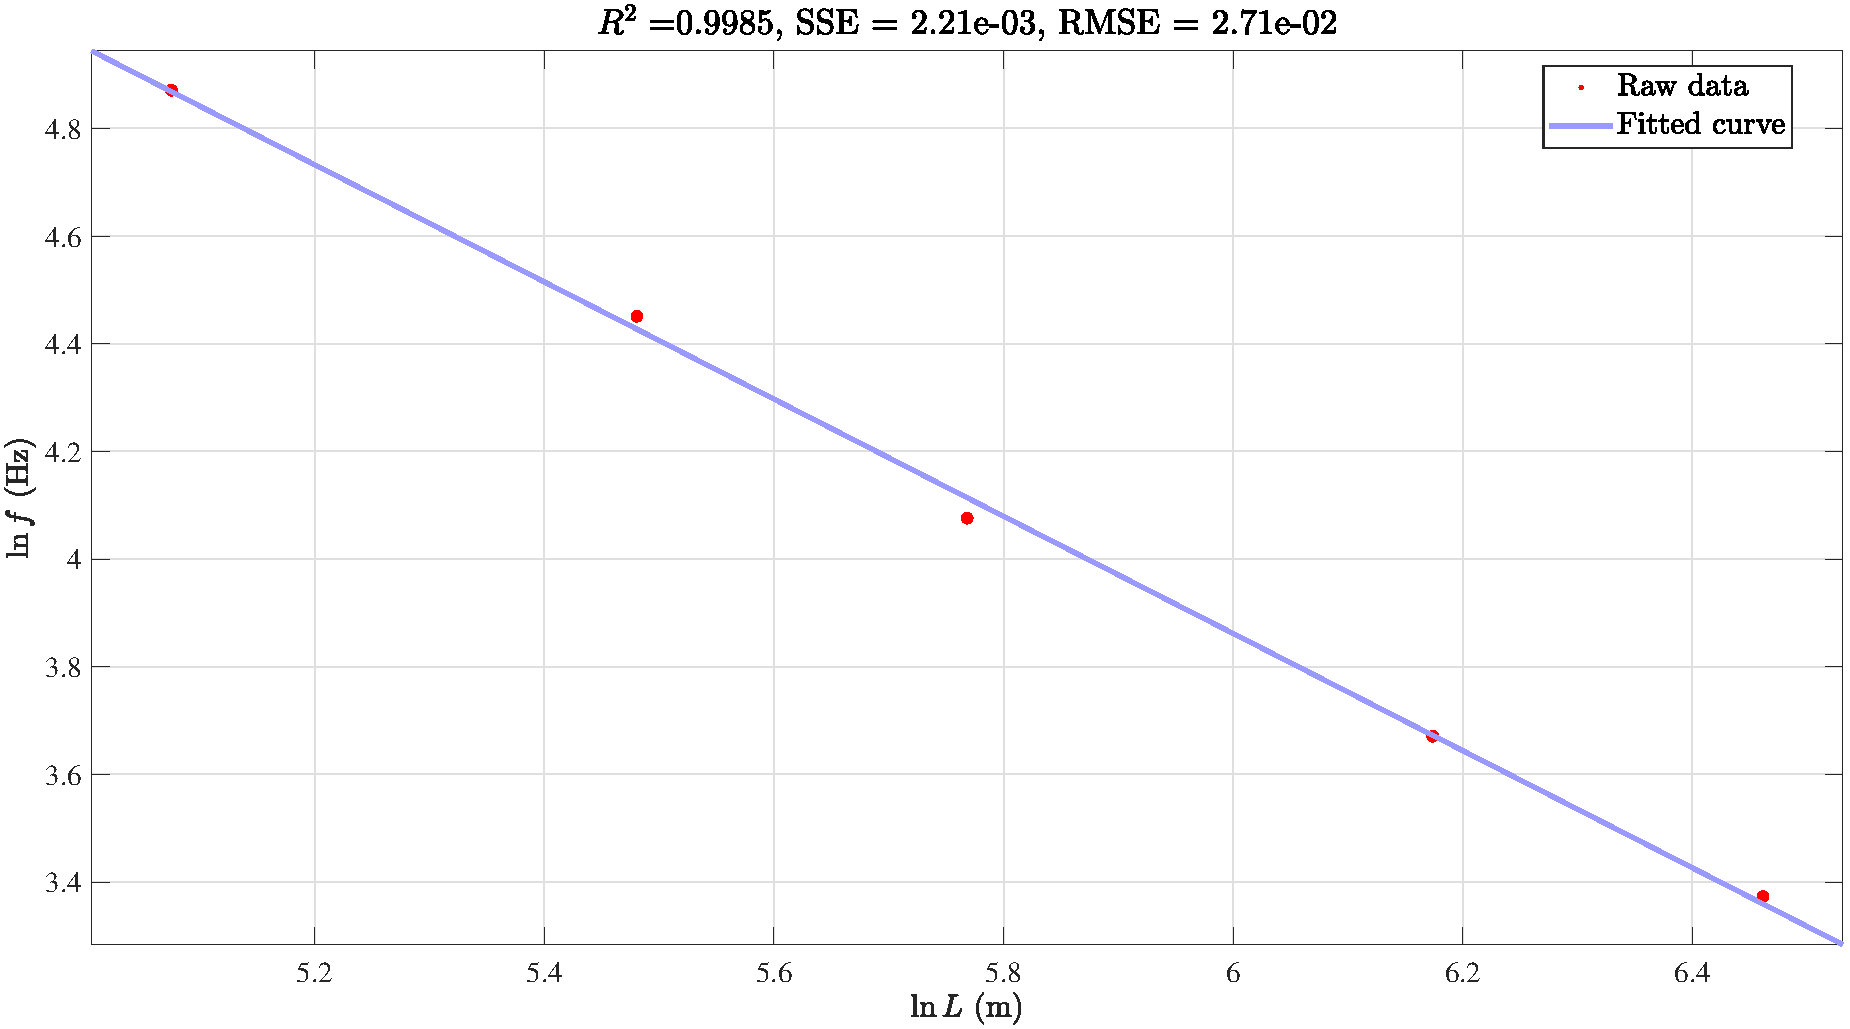
\includegraphics[width=0.9\columnwidth]{assets/3.pdf}
    \caption{有效长度与基频的线性拟合}
    \label{有效长度与基频的线性拟合}
\end{figure}

%	理论上上表第三行中数据应在误差允许范围内可看作相等,但实际数据中前两项相等,后三项相等,可能的原因是当弦线有效长度减小后,激振源与接收器距离过近,激振源发出信号由接收器直接接收对基频的测定造成了干扰使得实验结果出错。

\subsubsection{频率与张力的关系}
将琴码分别放置在200\,mm和600\,mm位置,固定有效长度$ L=400\,\mathrm{mm} $,将砝码分别放置在1-5格,测量不同拉力下的基频$ f_1 $。数据记录见表 \ref{频率与张力的关系}。
根据实验数据,在 Matlab 中用最小二乘法求出拟合直线,如下图所示:
\begin{figure}[H]\centering
    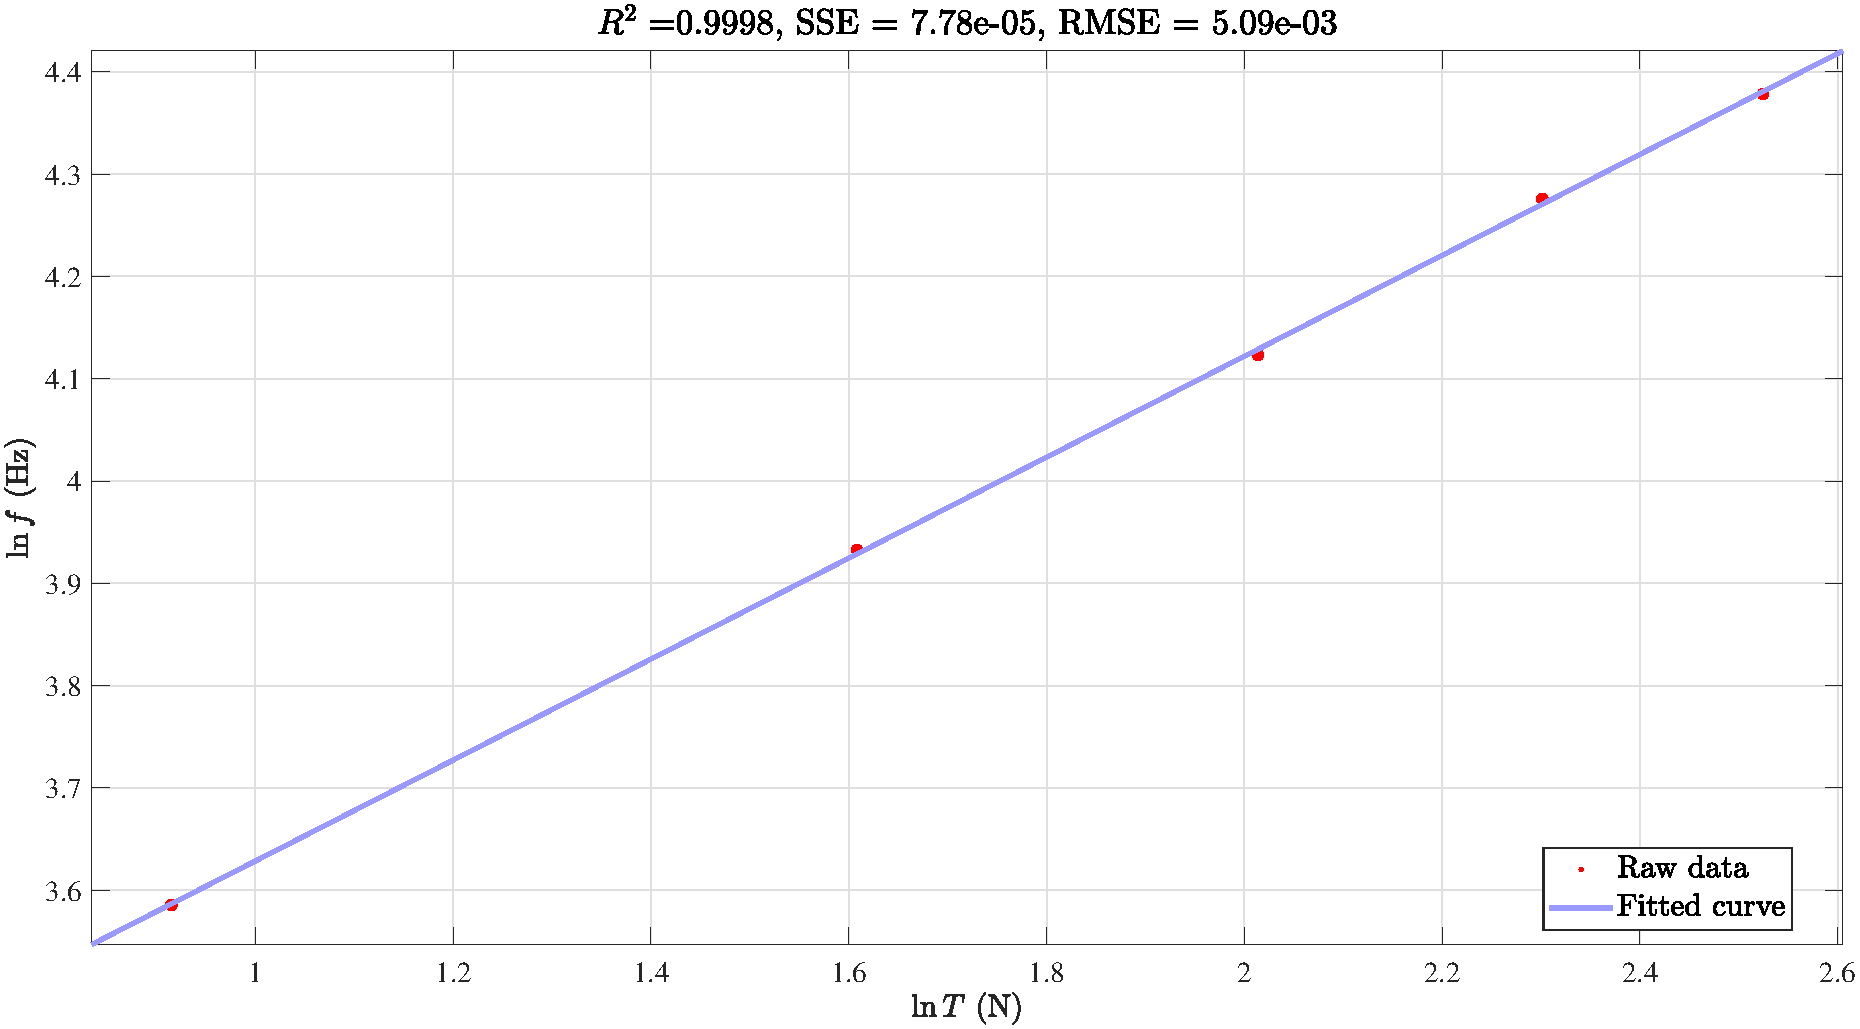
\includegraphics[width=0.9\columnwidth]{assets/4.pdf}
    \caption{频率与张力的线性拟合}
\end{figure}
图中拟合直线为:
\begin{equation}
y = 0.4934 \,x + 3.135
\end{equation}
由拟合直线斜率$ k=0.4934\approx\frac12 $可知$ \ln f_1=\frac 12\ln T+C $(此时$ C $为常数),即$ f_1\propto\sqrt{T} $.

\begin{table}[H]\centering
    %\renewcommand{\arraystretch}{1.5} % 调整行间距为 1.5 倍
    %\setlength{\tabcolsep}{1.5mm} % 调整列间距
    \caption{频率与张力的关系}
    \label{频率与张力的关系}
\begin{tabular}{cccccccccc}\toprule
    张力 $T$ (N)&2.4969&    4.9938&    7.4908&    9.9877&   12.4846\\
    \midrule
    基频 $f_1$ (Hz)&36.07&   51.04&   61.76&   71.93&   79.71\\
    $\ln T$&0.9151&   1.6082&    2.0137&    2.3014&    2.5245\\
    $\ln f_1$&3.5855&   3.9326&    4.1233&    4.2757&    4.3784\\
    \bottomrule
\end{tabular}
\end{table}

\subsubsection{频率与线密度之间的关系}
将琴码分别放置在200\,mm和600\,mm位置,固定有效长度$ L=400\,\mathrm{mm} $,将砝码放置在\textbf{第 3 格},通过共享数据得到不同粗细琴弦的基频。数据记录如表 \ref{不同线密度琴弦的基频} 所示:
上表中,(弦号, 直径, 线密度, 基频) = (5, 0.388 mm, 0.946 g/m, 55.76 Hz) 的一组数据明显异常,可能是由于实验操作不当导致的,故而在数据处理时应予以排除。根据剩余实验数据,在 Matlab 中用最小二乘法求出拟合直线,如下图所示:
\begin{figure}[H]\centering
    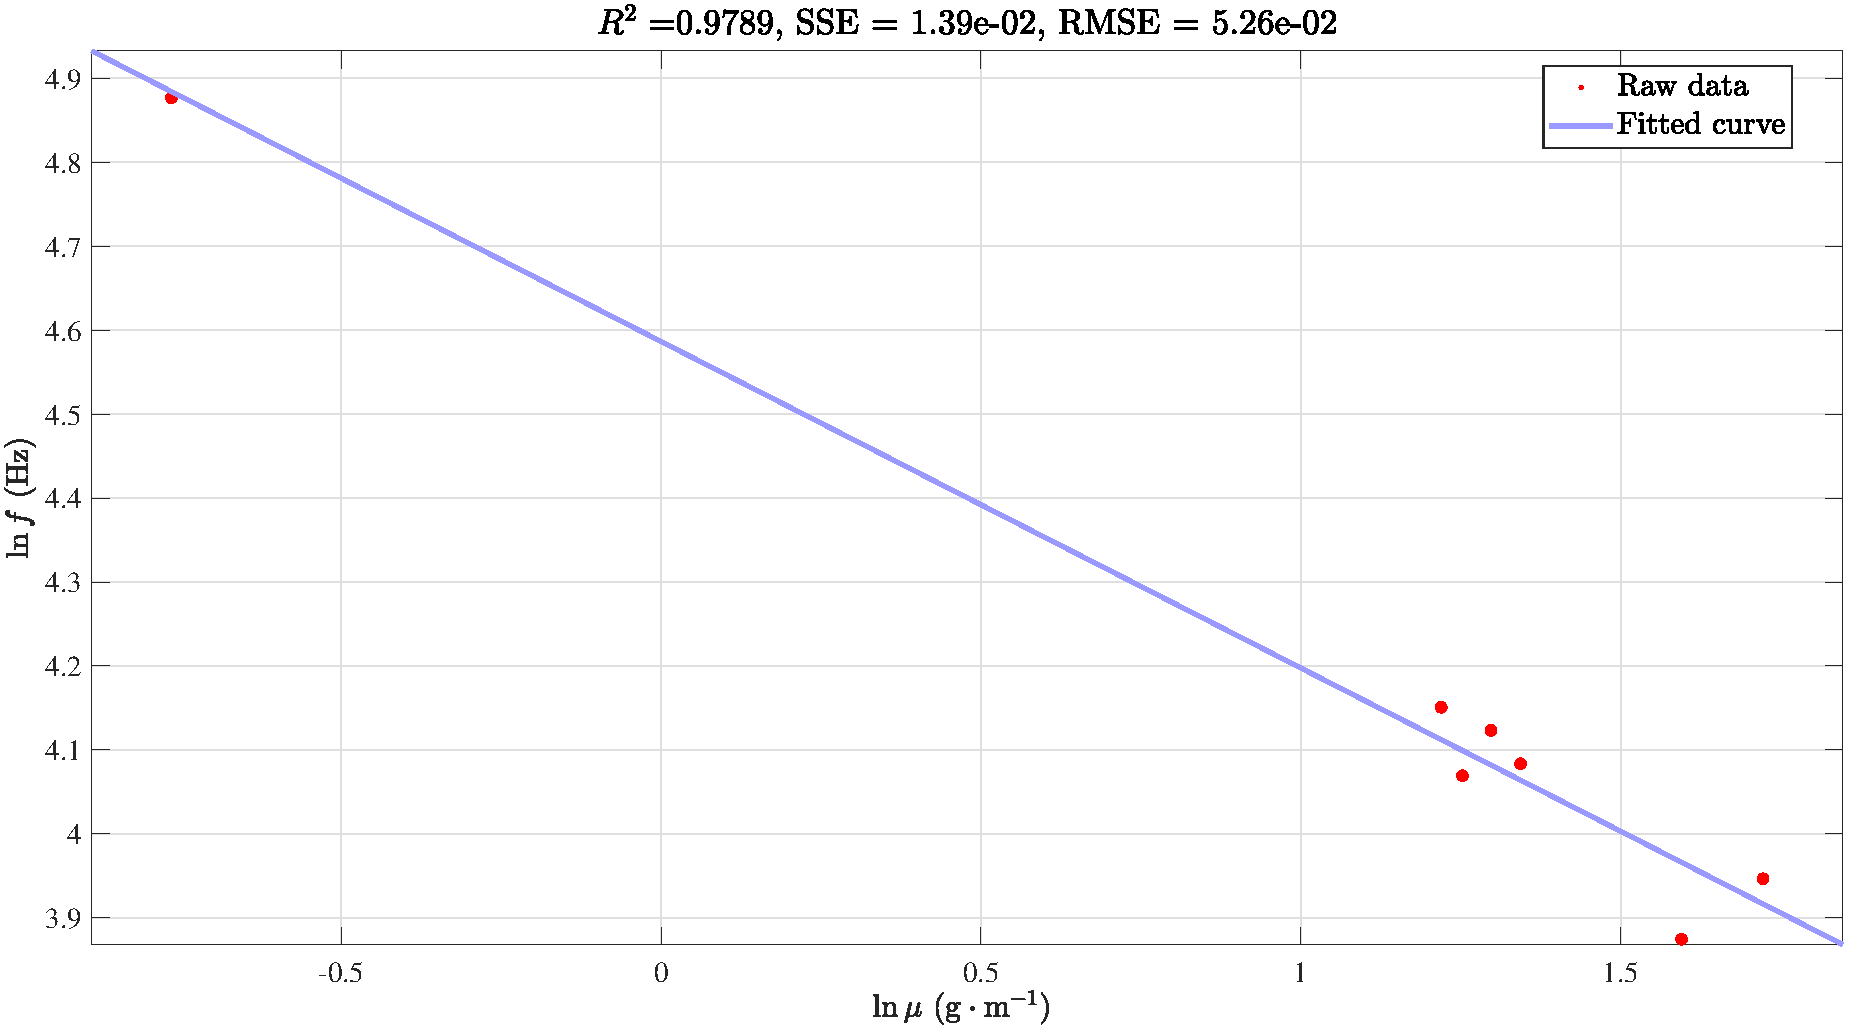
\includegraphics[width=0.9\columnwidth]{assets/5.pdf}
    \caption{频率与张力之间的线性拟合 (去除一个异常值)}
\end{figure}
其中拟合函数为:
\begin{equation}
y = -0.3889 \, x + 4.586
\end{equation}
可以看到,斜率 $k = -0.3889$ 与理论值 - 0.5 差异较大。但是,如果我们再去除 (弦号, 直径, 线密度, 基频) = (4, 0.235 mm, 0.465 g/m, 131.21 Hz) 的数据,再次进行拟合,得到的拟合直线如下:
\begin{equation}
y = -0.4659 \, x + 4.696
\end{equation}
\begin{figure}[H]\centering
    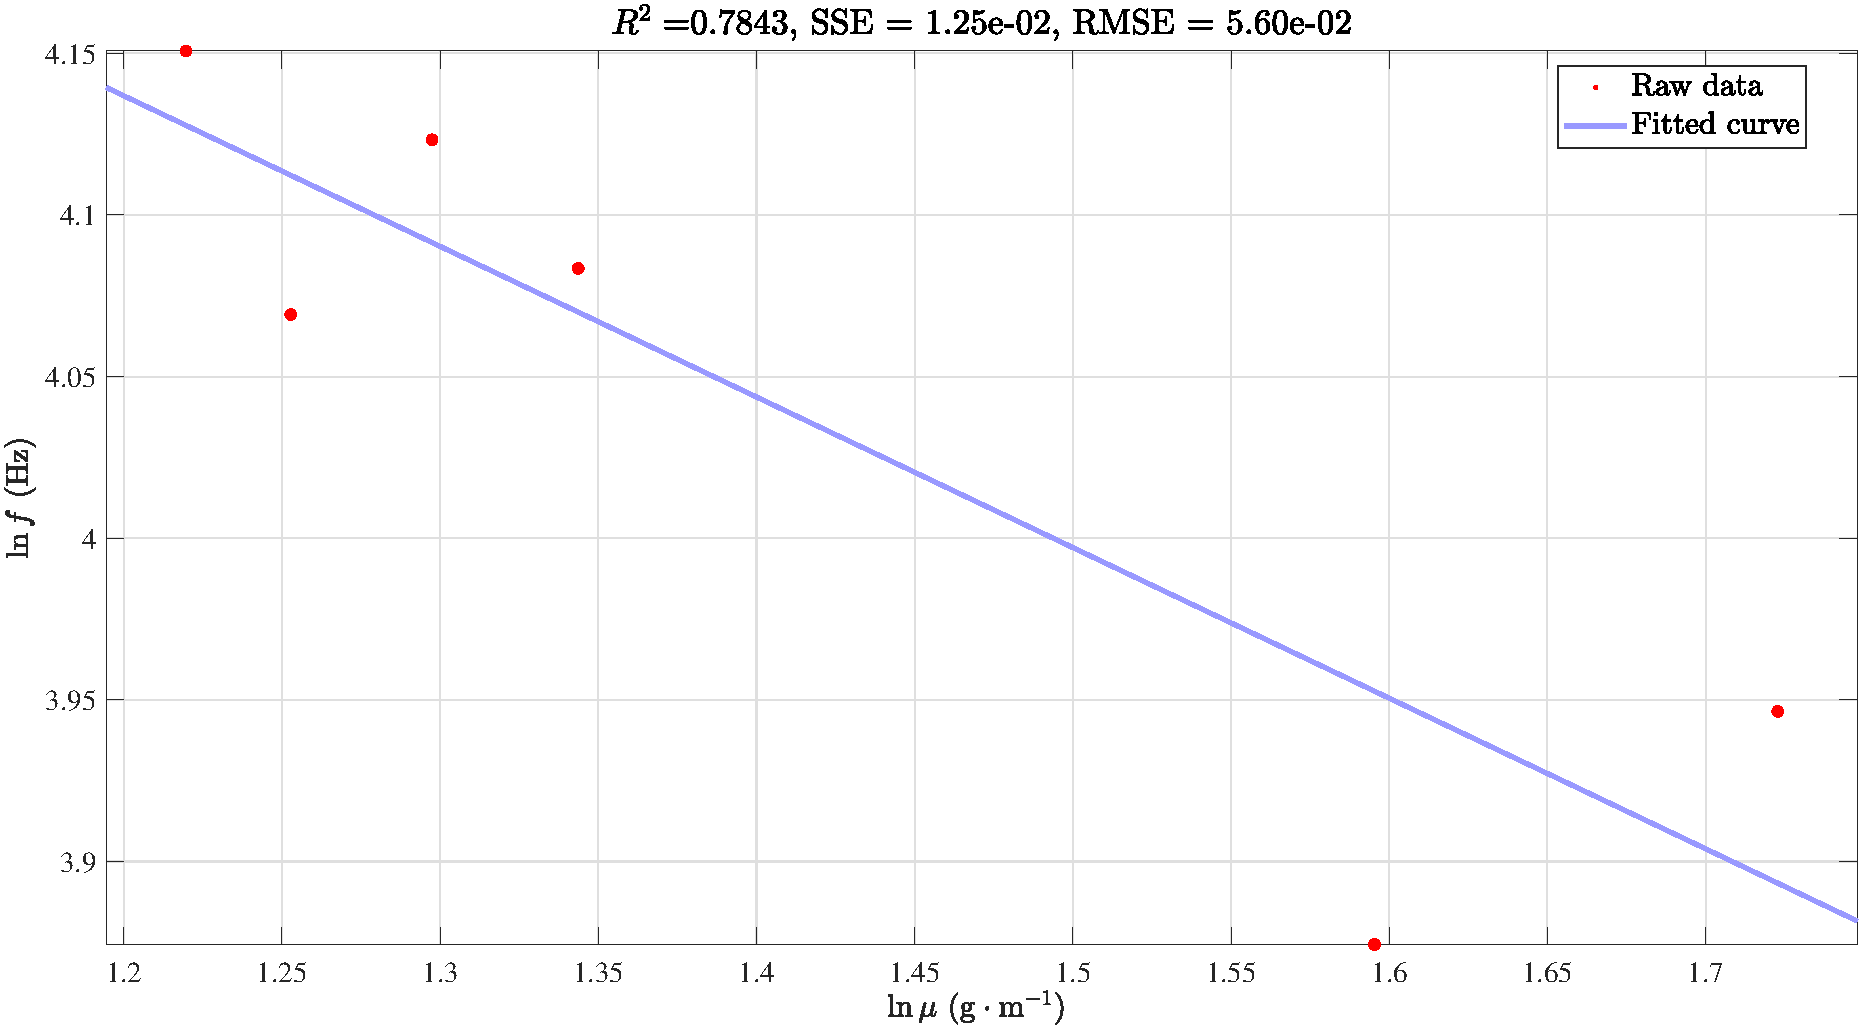
\includegraphics[width=0.9\columnwidth]{assets/6.pdf}
    \caption{频率与张力之间的线性拟合 (去除两个数据点)}
\end{figure}
此时,由拟合直线斜率$ k=-0.4659\approx- 0.5 $可知$ \ln f_1=-\frac12\ln\mu+C $(此时$ C $为常数),即$ f_1\propto\frac{1}{\sqrt \mu} $.

\begin{table}[H]\centering
    %\renewcommand{\arraystretch}{1.5} % 调整行间距为 1.5 倍
    %\setlength{\tabcolsep}{1.5mm} % 调整列间距
    \caption{不同线密度琴弦的基频}
    \label{不同线密度琴弦的基频}
\begin{tabular}{cccccccccc}\toprule
    弦号 & 6 & 1 & 3 & 7 & 5 & 4 & 10 & 9  \\
    \midrule
    直径 $d$ (mm) 
    & 0.883 & 1.070 & 1.000 & 0.771 & 0.388 & 0.235 & 0.885 & 0.43  \\
    线密度 $\mu$ ($\mathrm{g}\cdot m^{-1}$)
    & 3.66 & 4.93 & 5.60 & 3.50 & 0.95 & 0.47 & 3.83 & 3.39  \\
    基频 $f_1$ (Hz) 
    & 61.76 & 48.15 & 51.75 & 58.51 & 55.76 & 131.21 & 59.35 & 63.48 \\
    \bottomrule
\end{tabular}
\end{table}


\section{第二部分:测定介质中的声速}

\subsection{实验目的}
\begin{enumerate}
\item 利用驻波法测定波长;
\item 利用相位法测定波长;
\item 计算超声波在空气中和水中的传播速率。
\end{enumerate}

\subsection{实验器材}
SW-2型声速测量仪,信号发生器,示波器。

\subsection{实验原理}
\subsubsection{利用驻波法测声速}
\begin{enumerate}
\item 将信号发生器输出的正弦电压信号经超声发射换能器电声转换为超声波发射出去,经由接受换能器声电转换为电压信号,传入示波器。
\item 若接收面与发生面严格平行,入射波在接收面上垂直反射,入射波、反射波相互干涉形成驻波,此时两换能器之间距离恰好等于其声波半波长的整数倍。声驻波中,可通过接收换能器端面声压的变化来判断超声波是否形成驻波。
\item 转动鼓轮,改变两只换能器间的距离,在一系列特定的距离上,将会出现稳定驻波,记录出现最大电压数值时标尺上的刻度,相邻两次最大值对应的刻度值之差即为半波长。
\item 已知频率$ f $,经由上述方式测得波长$ \lambda $,则可根据公式$ v=\lambda f $可算出超声波的传播速度$ v $。
\end{enumerate}







\subsubsection{利用相位法测声速}
\begin{enumerate}
\item 将发射波和接收波同时输入示波器,以X-Y模式显示,两波的频率相同,相位不同。党接受点与发射点的距离变化恰等于波长的整数倍时,相位差为$ 2\pi $的整数倍,等效为相位差为$ 2\pi $。
\item 实验过程中,通过改变发射器和接收器之间的距离,观察李萨如图形的变化进而观察相位变化,当相位改变$ \pi $时,相应距离的改变量即为半波长。频率已知,根据公式$ v=\lambda f $可求出波速。
\item 相位变化时,李萨如图形的变化如下图所示:
\begin{figure}[H]\centering
    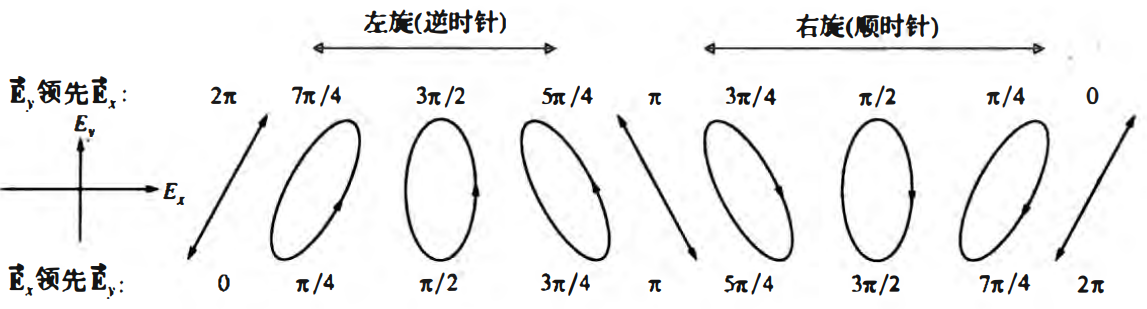
\includegraphics[width=0.8\columnwidth]{assets/5.5/5.1 主轴为 y.png}
    \caption{不同相位下的李萨如图形}
\end{figure}
\end{enumerate}
具体而言,我们有:
\begin{figure}[H]\centering
    \begin{subfigure}[b]{0.24\columnwidth}\centering
        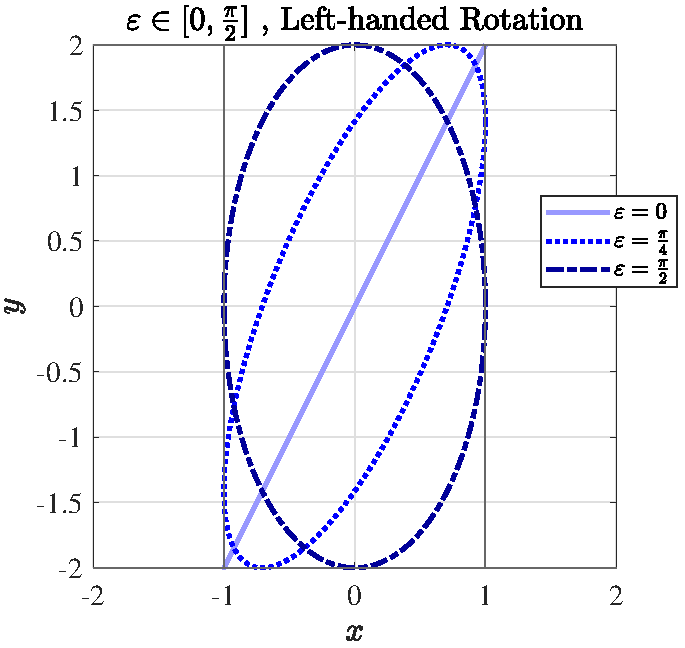
\includegraphics[height=110pt]{assets/5.5/2024-11-20_15-43-12.pdf}
        \caption{$\varepsilon \in [0, \frac{\pi}{2}]$, Left Rotation}
    \end{subfigure}
    \begin{subfigure}[b]{0.24\columnwidth}\centering
        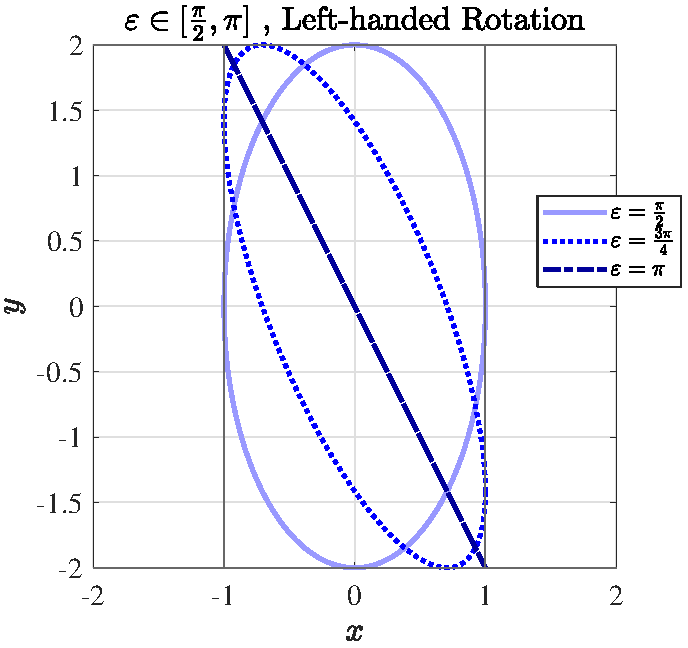
\includegraphics[height=110pt]{assets/5.5/2024-11-20_15-43-14.pdf}
        \caption{$\varepsilon \in [\frac{\pi}{2}, \pi]$ , Left Rotation}
    \end{subfigure}
    \begin{subfigure}[b]{0.24\columnwidth}\centering
        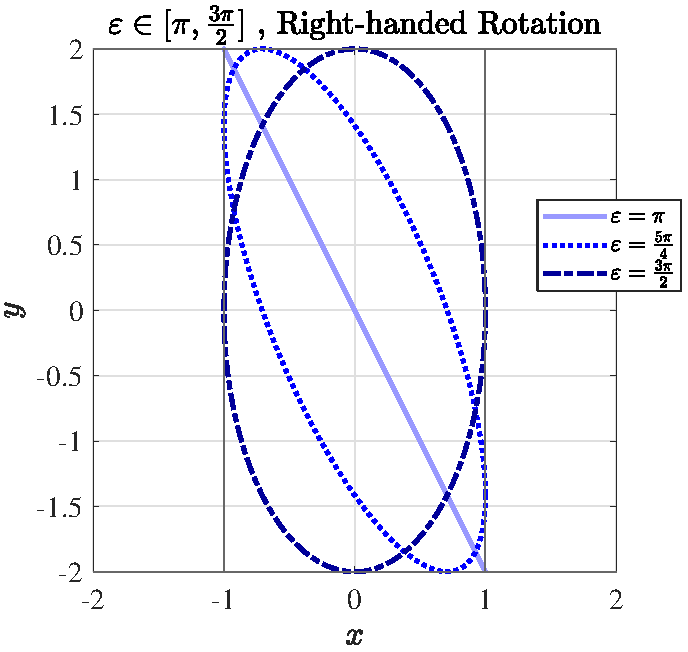
\includegraphics[height=110pt]{assets/5.5/2024-11-20_15-43-16.pdf}
        \caption{$\varepsilon \in [\pi, \frac{3\pi}{2}]$ , Right Rotation}
    \end{subfigure}
    \begin{subfigure}[b]{0.24\columnwidth}\centering
        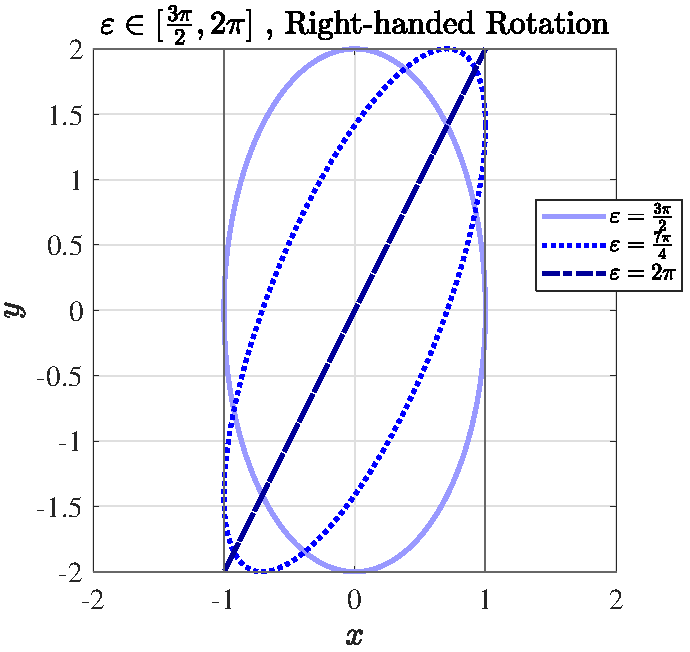
\includegraphics[height=110pt]{assets/5.5/2024-11-20_15-43-18.pdf}
        \caption{$\varepsilon \in [\frac{3\pi}{2}, 2\pi]$ , Right Rotation}
    \end{subfigure}
    \caption{李萨如图形随相位的变化关系 (主轴为 $y$)}
\end{figure}

\subsubsection{声速的理论值}
利用声速在空气中的理论公式可以计算空气中声速的理论值:
\begin{equation}
v=v_0\sqrt{\frac{T}{T_0}}=v_0\sqrt{1+\frac{t}{273.15}}
\end{equation}
其中$ T=(t+273.15)\,\mathrm K $,$ t $为摄氏温度,$ v_0=331.45\,\mathrm{m/s} $为$ 0 $\,\textcelsius 时的声速。

\subsection{实验内容}
\begin{enumerate}
\item 利用驻波法测超声波在空气中的波速;
\item 利用相位法测超声波在空气中的波速;
\item 利用驻波法或相位法测超声波在水中的波速;
\item 利用逐差法处理实验数据。
\end{enumerate}

\subsection{实验结果与数据处理}
\subsubsection{驻波法测超声波在空气中的声速}
实验时室温为$ t=28.0 $\,\textcelsius,调节信号发生器产生频率$ f=40\,\mathrm{kHz} $的正弦波,连接实验器材,调节声速测量仪鼓轮,用驻波法测量得到数据如下:
\begin{table}[H]\centering
    %\renewcommand{\arraystretch}{1.5} % 调整行间距为 1.5 倍
    %\setlength{\tabcolsep}{1.5mm} % 调整列间距
    \caption{驻波法求空气中声波波速}
    \label{驻波法求空气中声波波速}
\resizebox{\columnwidth}{!}{
    \begin{tabular}{ccccccccccccccc}\toprule
        序号 & 1 & 2 & 3 & 4 & 5 & 6 & 7 & 8 & 9 & 10 \\
        \midrule
        刻度值 (mm) & 24.423&	28.808&	33.315&	37.854&	42.221&	46.557	&50.920	& 55.031&	59.542&	63.753\\
        \bottomrule
    \end{tabular}
}
\end{table}
利用逐差法处理上表数据可求得波长$ \lambda $为
\begin{equation}
\lambda=\frac{\sum_{i=1}^{5}2(L_{i+5}-L_i)/5}{5} = 8.7346 \ \mathrm{mm}
\end{equation}
故而根据$ v=\lambda f $,可求得实验波速 $v_{\text{expe}}$,依据室温 $t = 28.0 \,\textcelsius$,可以求得理论波速 $v_{\text{theo}}$。实验波速 $v_{\text{expe}}$、理论波速 $v_{\text{theo}}$ 及它们的相对误差汇总如下:
\begin{equation}
    v_{\text{expe}} = 349.3824 \ \mathrm{m \cdot s^{-1}},\quad 
    v_{\text{theo}} = 348.0237 \ \mathrm{m \cdot s^{-1}},\quad 
    \eta = \frac{v_{\text{expe}} - v_{\text{theo}}}{v_{\text{theo}}} = 0.3904\ \%
\end{equation}
可以看到,理论值和实验值符合得非常好。

\subsubsection{相位法测超声波在空气中的声速}
室温与超声波与上小节相同,用相位法取$ \Delta\varphi=2\pi $(间隔一个波长)时的位置数据如下:
\begin{table}[H]\centering
    %\renewcommand{\arraystretch}{1.5} % 调整行间距为 1.5 倍
    %\setlength{\tabcolsep}{1.5mm} % 调整列间距
    \caption{相位法求空气中声波波速}
    \label{相位法求空气中声波波速}
\resizebox{\columnwidth}{!}{
    \begin{tabular}{ccccccccccccccc}\toprule
        序号 & 1 & 2 & 3 & 4 & 5 & 6 & 7 & 8 & 9 & 10 \\
        \midrule
        刻度值 (mm) & 37.976&	46.697&	55.512&	63.862&	72.733&	81.501&	90.202&	99.220&	107.541&	116.421
        \\
        \bottomrule
    \end{tabular}
}
\end{table}

利用逐差法处理上述数据可求得波长$ \lambda $为
\begin{equation}
\lambda=\frac{\sum_{i=1}^{5}(L_{i+5}-L_i)/5}{5}= 8.7242 \ \mathrm{mm}
\end{equation}
实验波速 $v_{\text{expe}}$、理论波速 $v_{\text{theo}}$ 及它们的相对误差汇总如下:
\begin{equation}
    v_{\text{expe}} = 348.9680 \ \mathrm{m \cdot s^{-1}},\quad 
    v_{\text{theo}} = 348.0237 \ \mathrm{m \cdot s^{-1}},\quad 
    \eta = \frac{v_{\text{expe}} - v_{\text{theo}}}{v_{\text{theo}}} = 0.27132\ \%
\end{equation}
可以看到,理论值和实验值近乎完美符合。
\begin{figure}[H]\centering
    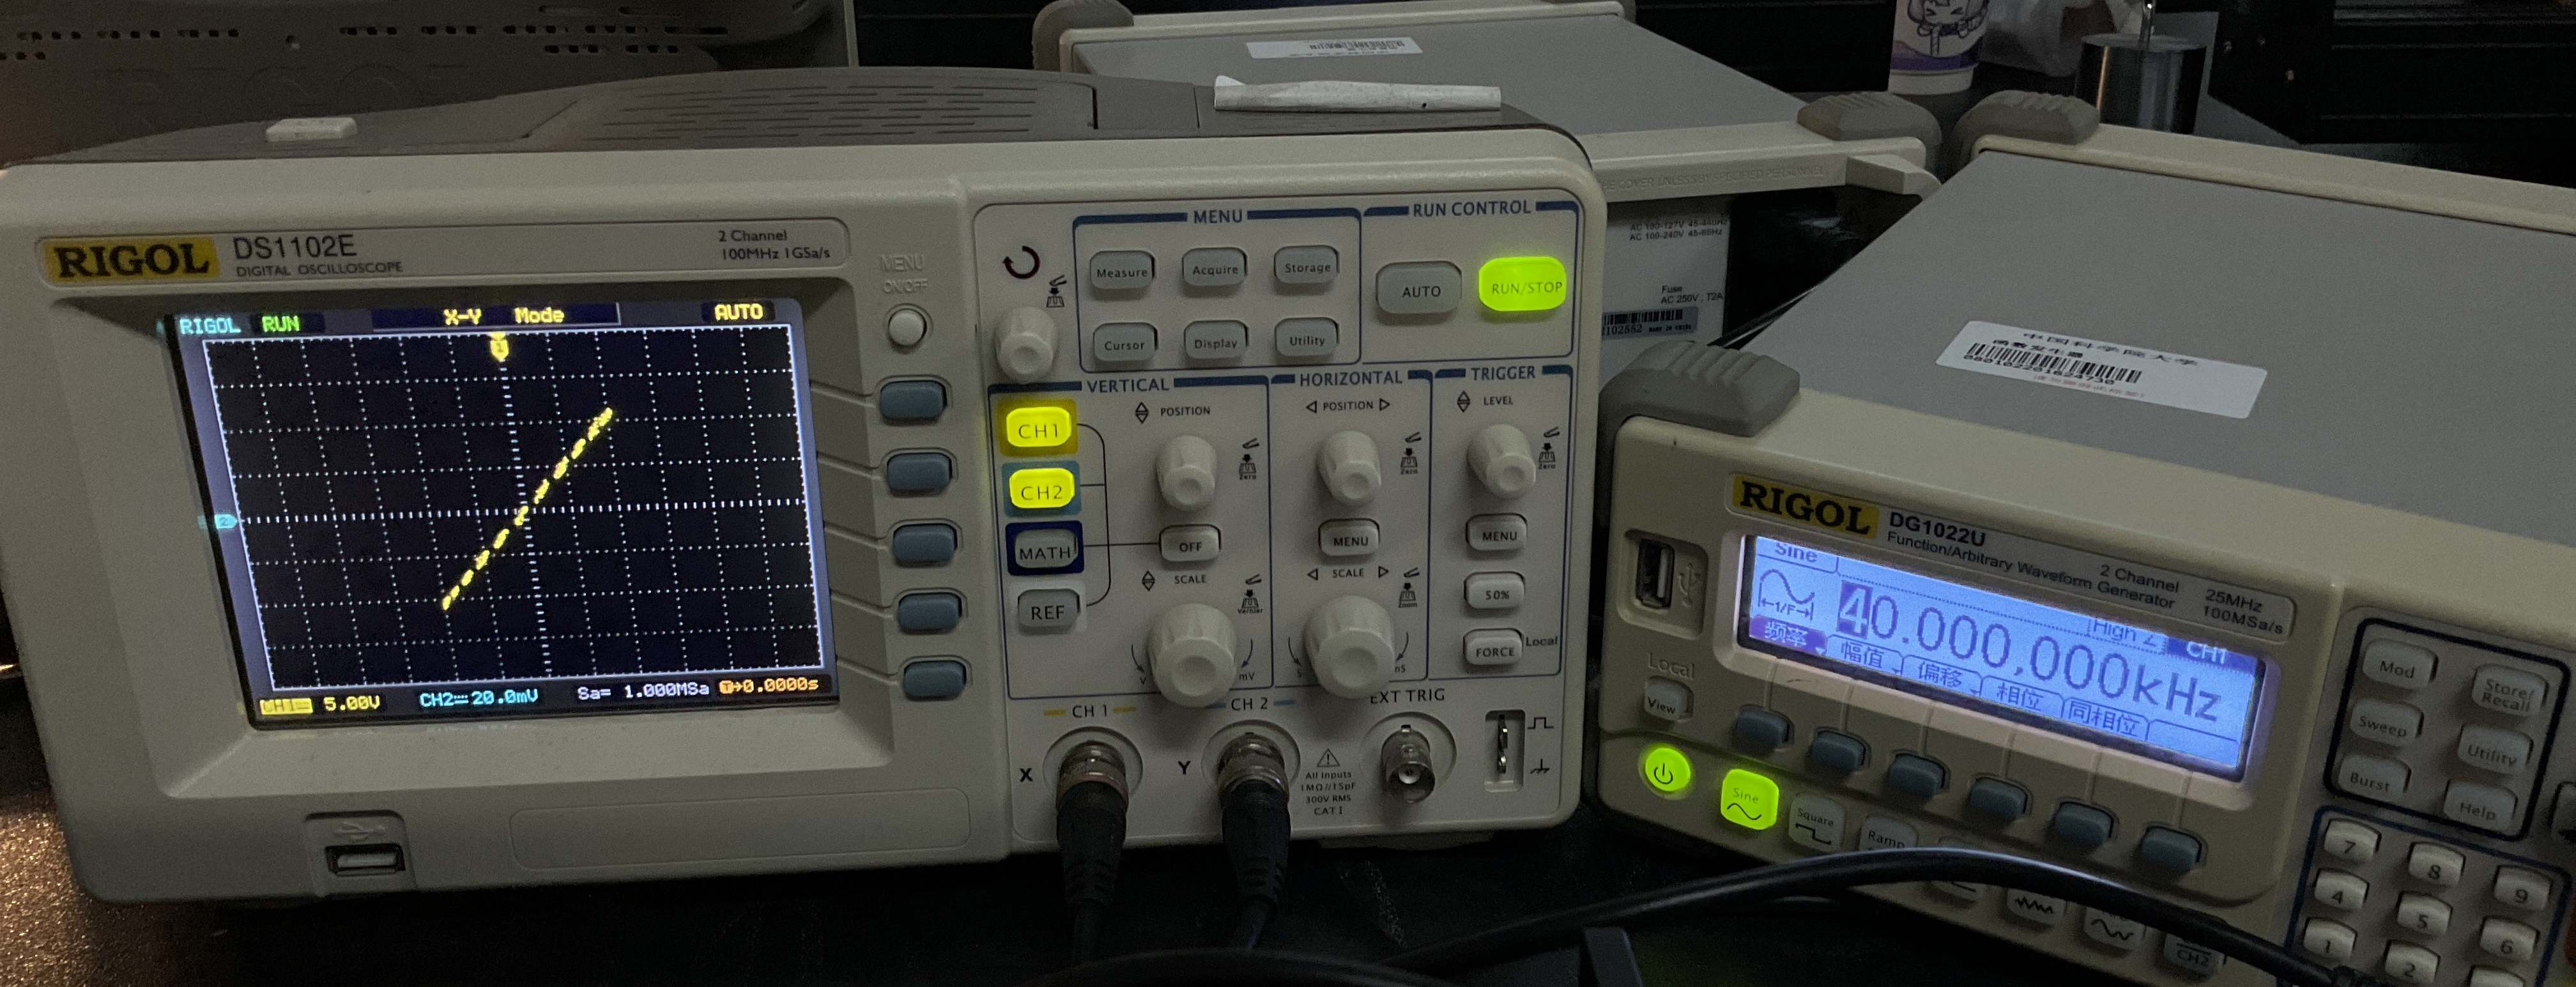
\includegraphics[width=0.75\columnwidth]{assets/相位法.jpg}
    \caption{相位法测波速实验照片}
\end{figure}


\subsubsection{相位法测超声波在水中的声速}
调节信号发生器产生频率$ f=1.8\,\mathrm{MHz} $的正弦波,连接实验器材,调节声速测量仪鼓轮,用相位法取$ \Delta\varphi=2\pi $(间隔一个波长)时的位置测得数据如下:
\begin{table}[H]\centering
    %\renewcommand{\arraystretch}{1.5} % 调整行间距为 1.5 倍
    %\setlength{\tabcolsep}{1.5mm} % 调整列间距
    \caption{驻波法求水中超声波波速}
    \label{驻波法求水中超声波波速}
\resizebox{\columnwidth}{!}{
    \begin{tabular}{ccccccccccccccc}\toprule
        序号 & 1 & 2 & 3 & 4 & 5 & 6 & 7 & 8 & 9 & 10 \\
        \midrule
        刻度值 (mm) & 53.899&	54.698&	55.417&	56.440&	57.310&	57.997&	58.792&	59.671&	60.580&	61.452
        \\
        \bottomrule
    \end{tabular}
}
\end{table}

利用逐差法处理上表数据可求得波长$ \lambda $为
\begin{equation}
\lambda=\frac{\sum_{i=1}^{5}(L_{i+5}-L_i)/5}{5}= 0.8291 \ \mathrm{mm}
\end{equation}
故而根据$ v=\lambda f $可求得波速为
\begin{equation}
    v_{\text{expe}} = 1492.4160\ \mathrm{m \cdot s^{-1}}
\end{equation}
水的折射率约为 $n = 1.3$,显然,这是一个超声波。


\section{思考题}

\subsection*{3.1 \ \ 调节振动源上的振动频率和振幅大小后对弦线振动会产生什么影响?}

弦线的振动由振源引起,弦线作受迫振动。调节振动源的频率时,会影响弦线上各点处前进波与反射波的干涉情况,一定条件下,驻波现象产生;调节振动源振幅大小,将影响弦线上各点的振动振幅,但对驻波现象是否产生没有影响。

在实验时,我还观察到,调节振源频率会导致示波器波形发生“移动”,这是因为振动还未稳定时,调频前的振动依然存在,调频后的新振动情况也出现,两振动发生干涉叠加,形成“移动”的复杂波形。

\subsection*{3.2 \ \  如何确定弦线上的波节点位置?}
通过肉眼观察,可以识别出弦线上振幅几乎为零(即无振动)的点,这些点就是波节点。如果需要更精确地定位波节点,可以通过调整接收器的位置,并观察示波器上的波形。在移动接收器的过程中,波形振幅最低的位置即为波节点。

\subsection*{3.3 \ \  在弦线上出现驻波的条件是什么?在实验中为什么要把弦线的振动调到驻波现在最稳定、最显著的状态?}
根据实验原理部分可知出现驻波的条件为$ n\lambda = 2L\;(n=1,2,3,\cdots) $,即有效长度是半波长的正整数倍。将弦线振动调节至驻波最稳定、最显著时弦线状态最接近驻波出现条件的状态,确保各点处前进波和反射波确实发生了有稳定相位差的稳定干涉,使得测得的基频更为准确。

如何实现驻波的最稳定和最显著状态?
根据实验原理,驻波产生的条件是 $ n\lambda = 2L\;(n=1,2,3,\cdots) $,意味着有效长度必须是半波长的整数倍。当弦线的振动被调整至最稳定和最显著的驻波状态时,弦线的状态将最接近驻波产生的条件,确保各点的前进波和反射波能够发生相位差稳定的干涉,从而提高准确性。

\subsection*{3.4 \ \ 在弹奏弦线乐器时,发出声音音调与弦线的长度、粗细、松紧程度有什么关系,为什么?}

在弹奏弦线乐器时,弦线长度越短、直径越小、琴弦越紧,发出声音的音调越高。弦线乐器的声音与弦线振动的频率$ f $正相关,而由实验过程验证过的实验原理$ \ln f=\frac12\ln T-\frac12\ln\mu-\ln\lambda $可得:$ f\propto\frac1L,\;f\propto\frac{1}{\sqrt\mu},\;f\propto\sqrt T $,即$ f $与弦线长度成负相关、弦线粗细成负相关、弦线松紧程度成正相关。

弹奏弦乐器时,弦线越短、直径越细、绷得越紧,发出的音调越高。弦乐器的音高与弦线的振动频率$ f $ 正相关,而根据实验原理中的 $ \ln f=\frac12\ln T-\frac12\ln\mu-\ln\lambda $,$ f\propto\frac1L,\;f\propto\frac{1}{\sqrt\mu},\;f\propto\sqrt T $,即 $ f $ 与弦线长度成反比、与弦线的粗细的 0.5 次方成反比、与弦线的松紧程度呈正相关。

\subsection*{3.5 \ \  若样品弦线与装置上的弦线直径略有差别,请判断是否需要修正,如何进行?}

需要进行修正。对于同种材料,其密度$ \rho $一定,考虑直径$ d_1,d_2 $不同的两条弦线,它们的线密度记为$ \mu_1,\mu_2 $,取相同长度$ l $,则有关系:
\begin{equation}
\frac{\frac{1}{4}\rho\pi d_1^2l}{\frac{1}{4} \rho\pi d_2^2l}=\frac{\mu_1l}{\mu_2l}\,\Longrightarrow\,\frac{d_1^2}{d_2^2}=\frac{\mu_1}{\mu_2}
\end{equation}
因此线密度$ \mu\propto d^2 $,故而修正方式为:测得样品弦线上的相关指标后测量装置弦线直径,计算并记录
\begin{equation}
    k=\frac{\text{装置弦线直径}}{\text{样品弦线直径}} 
\end{equation}
由样品弦线的线密度$ \mu $和直径$ d $可计算得到装置上弦线的线密度$ \mu'=k^2\mu $,也就是后续数据处理中实际使用的线密度$ \mu' $。


\subsection*{3.6 \ \  对于某一共振频率,增大或减小频率的调节过程中,振幅最大的频率位置往往不同,如何解释这一现象?}
驻波现象可以在一定的频率范围内观测到,但波列本身存在一定的不稳定性。实验中对频率的反复调节可能会引入回调误差,导致振幅最大的频率位置出现差异。在此实验中,由于需要反复调节频率以确定共振频率,这一现象是十分明显的,具体表现为:达到最大振幅且看似“稳定”的波形,经过足够长的时间后,其振幅又明显降低,这说明此时的频率并非真正的共振频率。

\section{实验总结与心得体会}
此次“驻波实验”实验共分为两个部分,实验过程均不复杂。在对横波的描述、波的干涉、驻波现象等知识有一定了解后,对于实验的理解体会也将不会构成难题。实验的一个重要思想是“对复杂的依赖关系取对数,以获得变量间的线性关系”,令我印象深刻;另一重点是数据的计算、拟合与逐差法分析,在处理的过程中,我也学到很多。

实验总体上是成功的,每个小节的实验都大致符合理论,实验数据和图像也具有较强的说服力。例如在“相位法测空气中声波波速”一小节中,实验测量值与理论标准值的相对误差仅为 $0.2713 \, \%$。

特别地,在本次实验,我利用了 Matlab 软件对实验数据作进一步的处理和分析,包括换算、拟合、可视化等,相比于常规数据处理和画图方法,这大大提高了数据分析处理的速度的准确度,也提高了作图的美观性。在今后的实验和研究工作中,我还会继续深入学习和应用类似地计算软件,增强自己的科学计算能力。科研不是考试,我们应该充分利用好自己能接触到的资源,合理使用工具,更高效地发展自身。

另外,这次实验让我感受到,实验“结束”并不意味着实验就已经完成,事实上这仅是数据测量的结束。在课后,我们还需要重新整理实验原理和过程,换算、分析、拟合实验数据,作出合适的数据图,解释可能存在的误差等。在根据已有数据求所需结果时,如何才能最大程度地利用已有数据,同时又尽可能地降低二次误差。上面这些内容都需要体现在最终的实验报告中,一点点累加起来,着实花费了我很多精力。

但最后回过头来,我认为一切都是值得的。当处理完毕的结果有力地验证了理论值时,当实验数据图像与理论较好地契合时,心中便迸发出无尽的喜悦,也深深感受到物理“理论与实验结合”的魅力\footnote{手写预习报告、原始数据记录表和 Matlab 源码附在附录中。}。

\newpage
\section*{附录 A\hspace*{20pt} 原始数据记录表}
\addcontentsline{toc}{section}{附录 A\hspace*{6pt} 原始数据记录表} 
\thispagestyle{fancy} 

\begin{figure}[H]\centering
    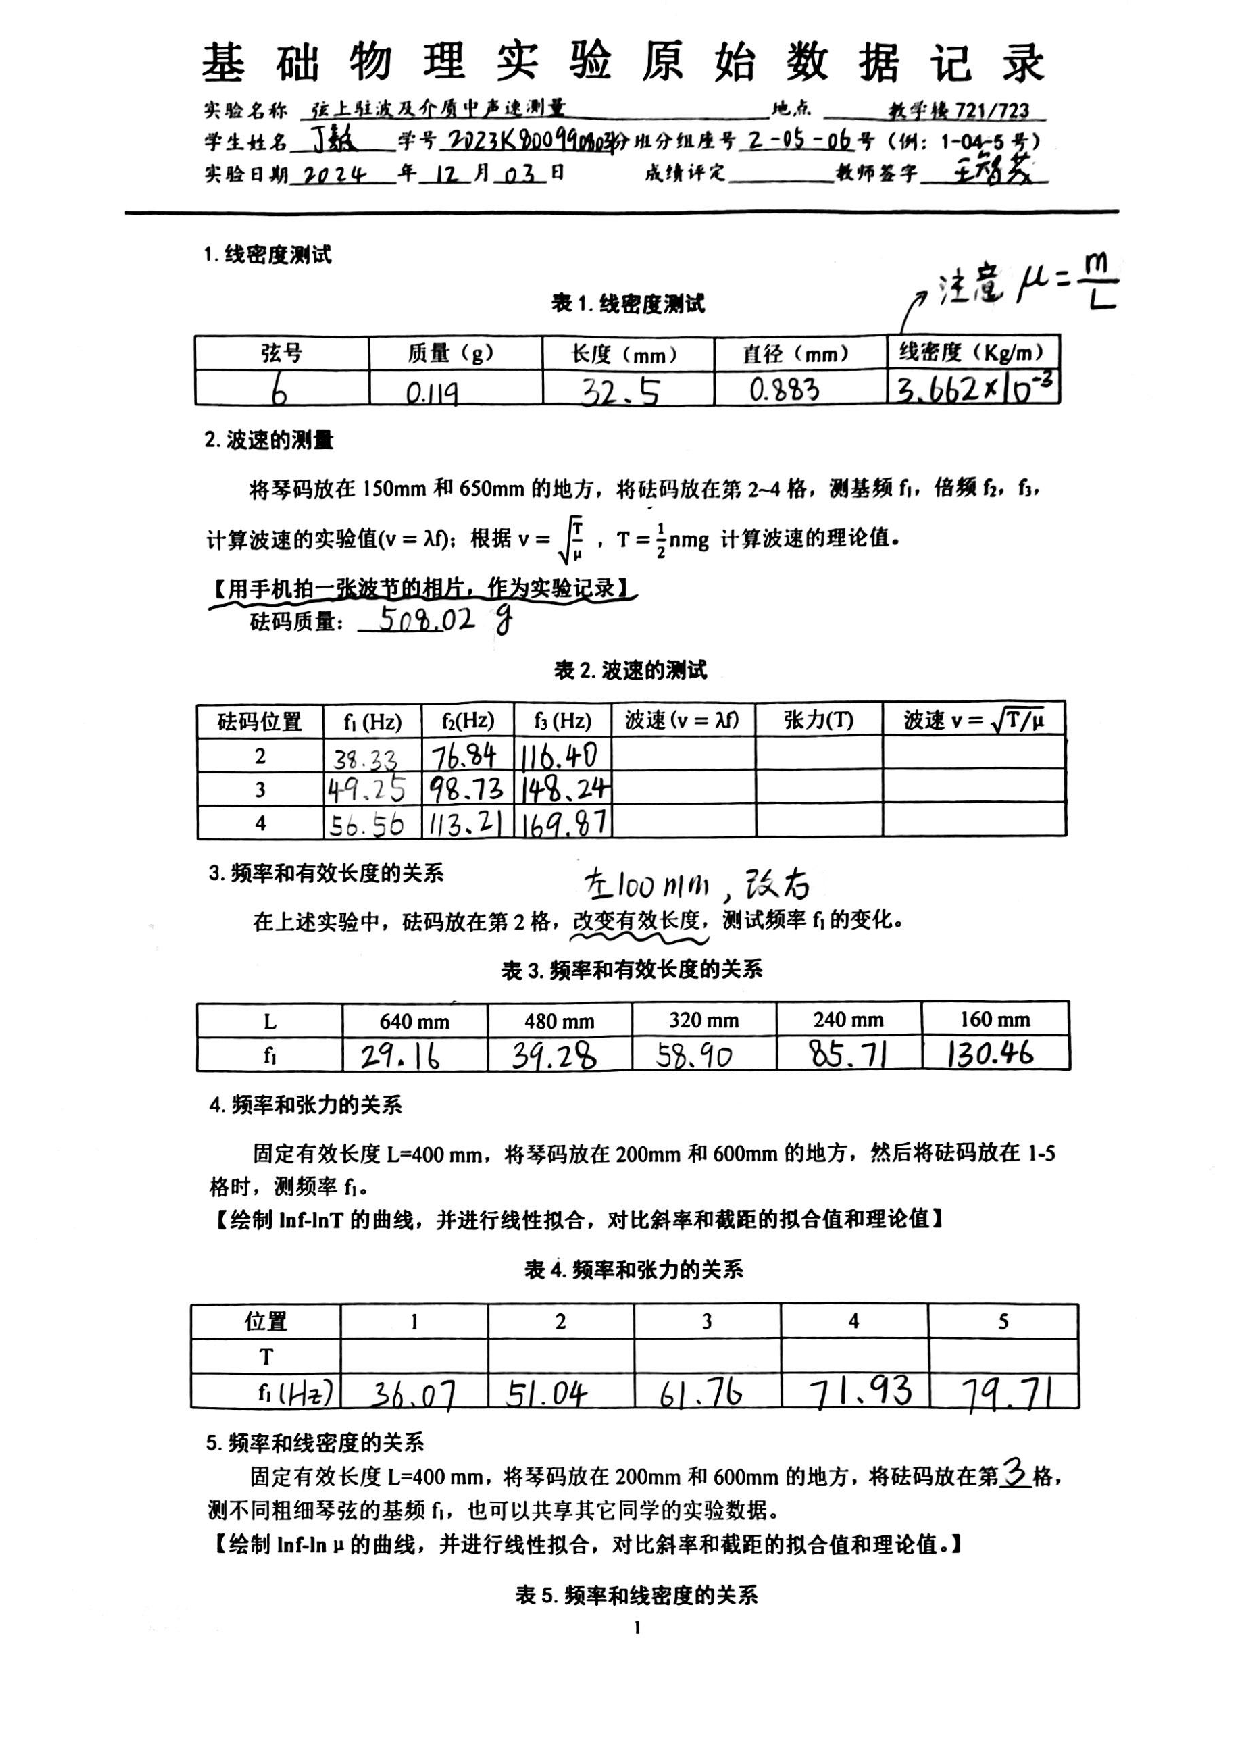
\includepdf[pages=1, width=480pt]{pdf/原始数据-2-05组-丁毅-驻波实验-2024.12.03-王智茂.pdf}
\end{figure}
\includepdf[pages={2}]{pdf/原始数据-2-05组-丁毅-驻波实验-2024.12.03-王智茂.pdf}

\section*{附录 B\hspace*{20pt} 手写预习报告}
\addcontentsline{toc}{section}{附录 B\hspace*{6pt} 手写预习报告} 
\thispagestyle{fancy} 

\begin{figure}[H]\centering
    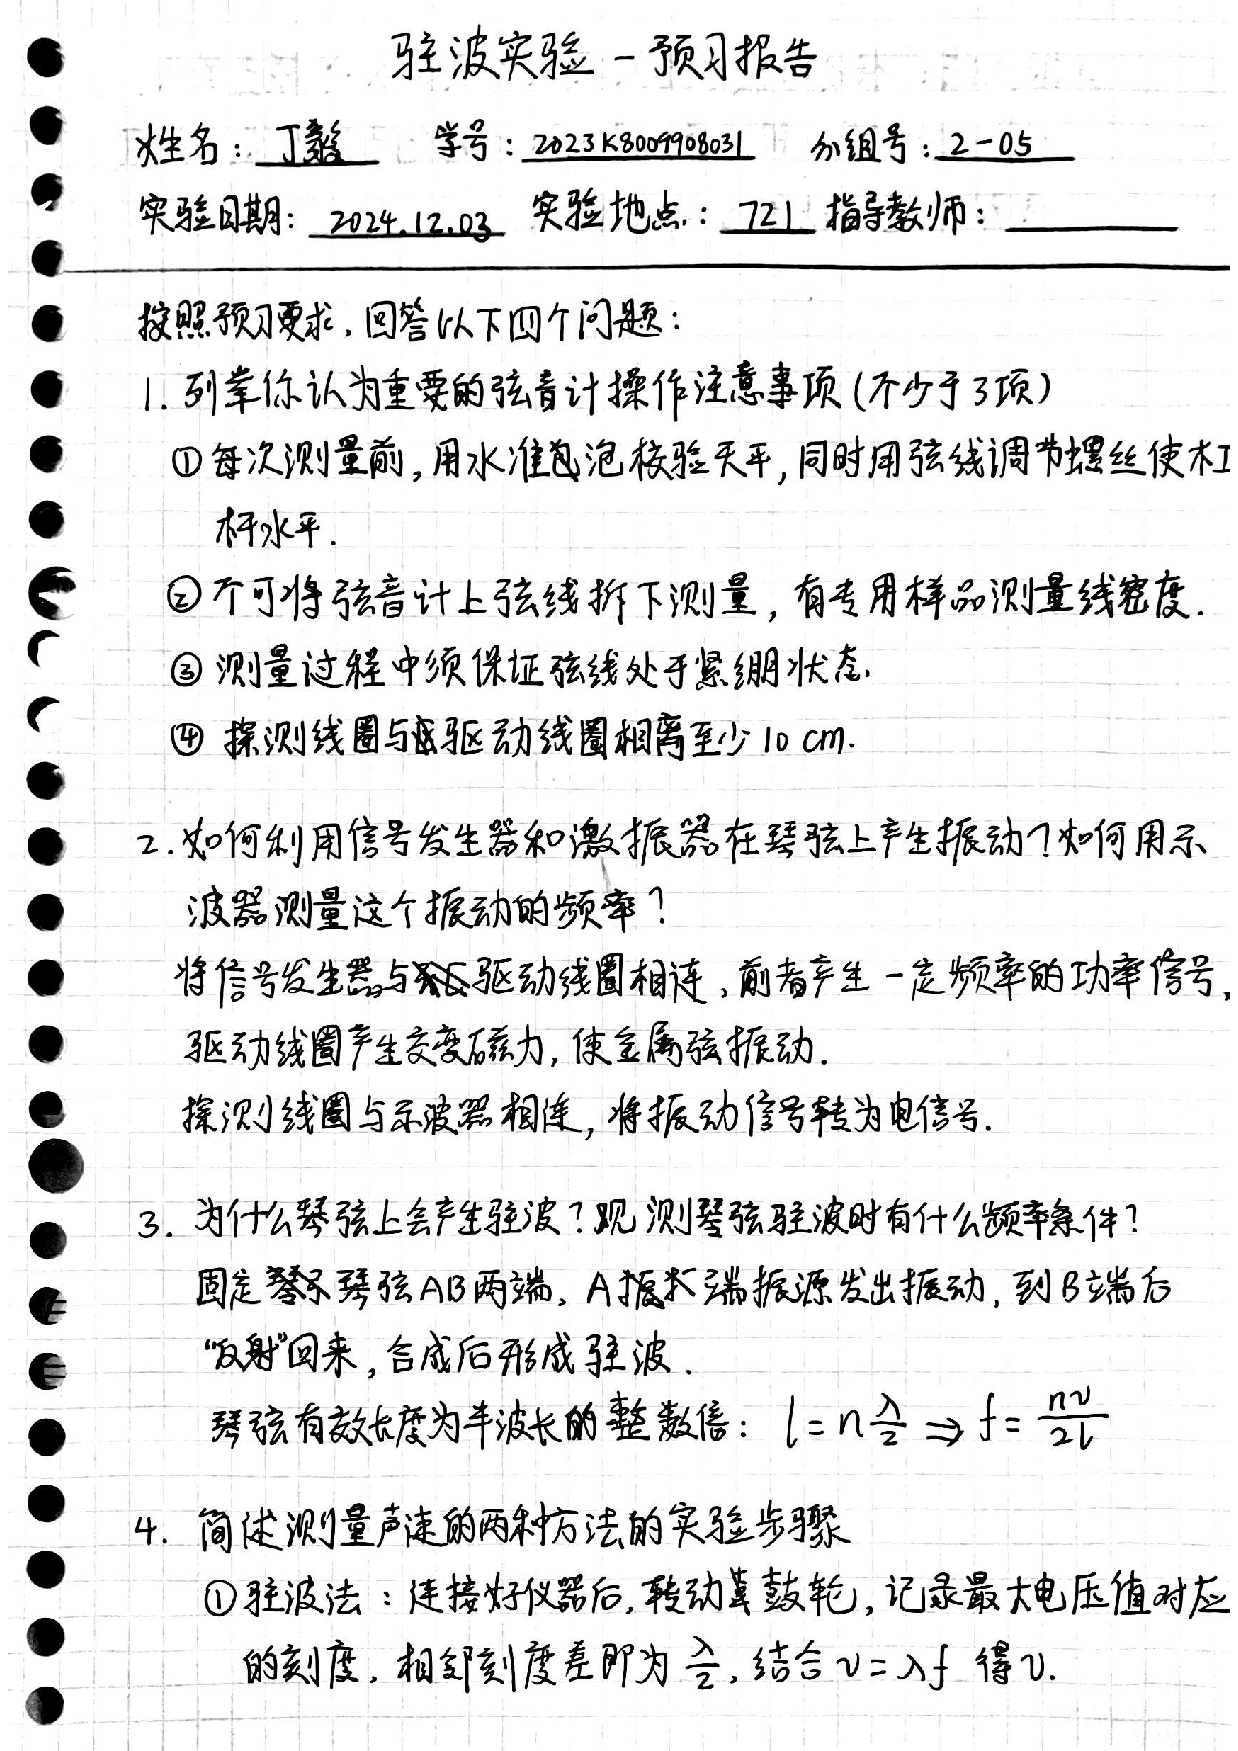
\includepdf[pages=1, width=480pt]{pdf/预习报告-2-05组-丁毅-驻波实验-2024.12.03.pdf}
\end{figure}
\includepdf[pages={2}]{pdf/预习报告-2-05组-丁毅-驻波实验-2024.12.03.pdf}

\section*{附录 C\hspace*{20pt} Matlab 源码}
\addcontentsline{toc}{section}{附录 C\hspace*{6pt} Matlab 源码} 
\thispagestyle{fancy} 
\lstinputlisting{d:/a_RemoteRepo/GH.MatlabCodes/本科课程代码/基础物理实验/Ex_3/Ex_03_mfile.m}



\end{document}

% VScode 常用快捷键:

% F2:                       变量重命名
% Ctrl + Enter:             行中换行
% Alt + up/down:            上下移行
% 鼠标中键 + 移动:           快速多光标
% Shift + Alt + up/down:    上下复制
% Ctrl + left/right:        左右跳单词
% Ctrl + Backspace/Delete:  左右删单词    
% Shift + Delete:           删除此行
% Ctrl + J:                 打开 VScode 下栏(输出栏)
% Ctrl + B:                 打开 VScode 左栏(目录栏)
% Ctrl + `:                 打开 VScode 终端栏
% Ctrl + 0:                 定位文件
% Ctrl + Tab:               切换已打开的文件(切标签)
% Ctrl + Shift + P:         打开全局命令(设置)

% Latex 常用快捷键:

% Ctrl + Alt + J:           由代码定位到PDF


